\part{Data Understanding}
    To successfully accomplish the objectives of this statistical analysis, it will be essential to gather data
    grouped under specific general attributes such as country, years. This data will be merged from various sources,
    considering the intricate nature of the analysis and the need to incorporate information related to each distinct
    feature.
    \\
    \\
    The primary data sources encompass renowned institutions. The utilization of these diverse sources promises to
    enhance and lend significance to the resulting model.
    \\
    \\
    Since there exists a multitude of data sources, I intend to address each dataset individually. However, certain
    repetitive processes will be elucidated in a more generalized manner.


    \section{\dsObesity}

        \subsection{\duCollectInitialData}

            Provided by The World Health Organization, this database encompasses information concerning the prevalence of obesity among adults with a BMI ≥ 30, which has been standardized for age. It serves to furnish data indicating the percentage of the population categorized as obese per country and per year.
            \\
            \\
            The dataset is conveniently accessible in various formats, ensuring ease of retrieval. Notably, it boasts a tabular representation in HTML, offering comprehensive insights into the entirety of the dataset.

        \subsection{\duDescribeTheData}
            \begin{figure}[H]
                \centering
                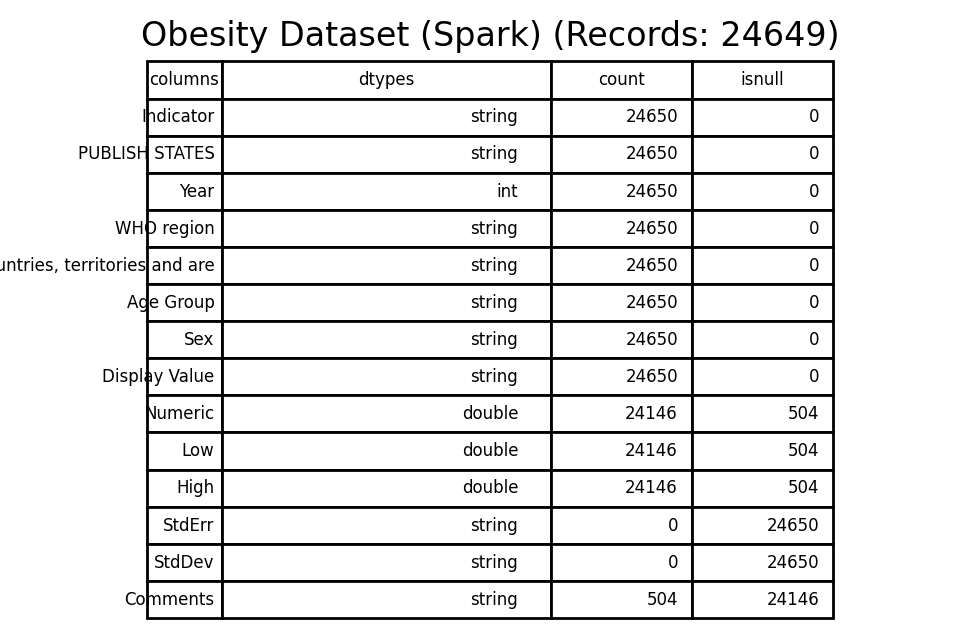
\includegraphics[scale=1.3]{images/du_obesity_dataset}
                \caption{Contains the information of percentages of obesity per country and year.}
                \label{fig:du-obesity-datasets}
            \end{figure}

            The \textit{\dsObesity} (\figurename~\ref{fig:du-obesity-datasets}) consists of 24,650 entries organized across 14 columns.

            \textbf{Text-based Columns:}
            \begin{enumerate}
                \item \textit{Indicator}: Describes the type of data indicator and has no missing values.
                \item \textit{PUBLISH STATES}: Indicates the publication status of the data, also with no missing entries.
                \item \textit{WHO region}: Specifies the WHO-defined region for the entry, complete with no missing values.
                \item \textit{Countries, territories and areas}: Lists the geographical areas relevant to the data, with no missing values.
                \item \textit{Age Group}: Describes the age group for the obesity measurement, again with no missing entries.
                \item \textit{Sex}: Indicates the sex of the individuals in the data and is complete with no missing values.
                \item \textit{Display Value}: The value to be displayed, and it is also complete with no missing data.
                \item \textit{Comments}: Contains additional comments, but most entries are missing with only 504 filled.
            \end{enumerate}

            \textbf{Numerical Columns:}
            \begin{enumerate}
                \item \textit{Year}: This integer column represents the year of data collection and has no missing entries.
                \item \textit{Numeric}: This float column represents some numerical value and has 504 missing entries.
                \item \textit{Low}: Represents the lower limit of a range, also a float column with 504 missing values.
                \item \textit{High}: Represents the higher limit of a range, another float column with 504 missing values.
                \item \textit{StdErr}: Represents the standard error but is completely missing with zero non-null entries.
                \item \textit{StdDev}: Represents the standard deviation, which is also completely missing with zero non-null entries.
            \end{enumerate}

            In summary, most of the text-based columns are complete with no missing values, while some numerical columns like \textit{StdErr} and \textit{StdDev} have all their entries missing. The \textit{Comments} text-based column also has a large number of missing entries.

        \subsection{\duExploreTheData}

            \begin{figure}[H]
                \centering
                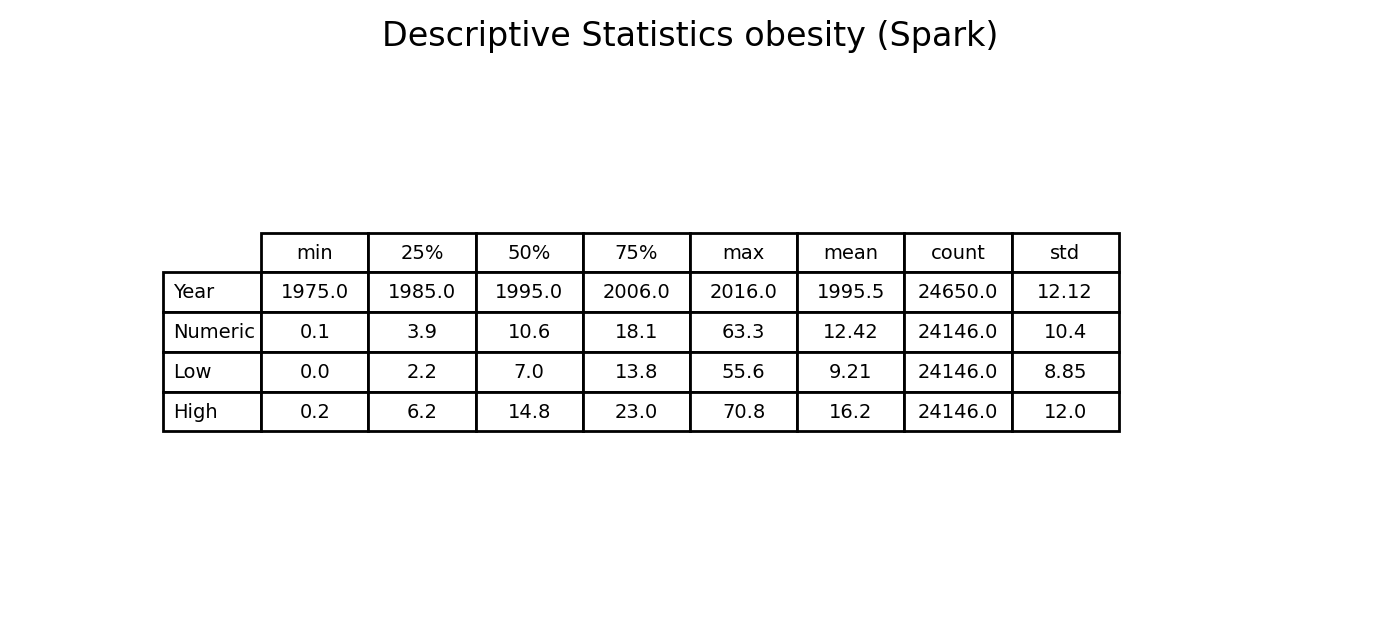
\includegraphics[scale=1]{images/du_obesity_summary}
                \caption{}
                \label{fig:du-obesity-summary}
            \end{figure}

            \figurename~\ref{fig:du-obesity-per-obe-countries-top-lw-20} showcases two boxplots stacked vertically. The top boxplot represents the percentages of obesity in the top 20 countries with the highest prevalence, while the bottom boxplot represents the same for the 20 countries with the lowest rates of obesity. These percentages are collected over a time span from 1975 to 2016.

            \begin{figure}[H]
                \centering
                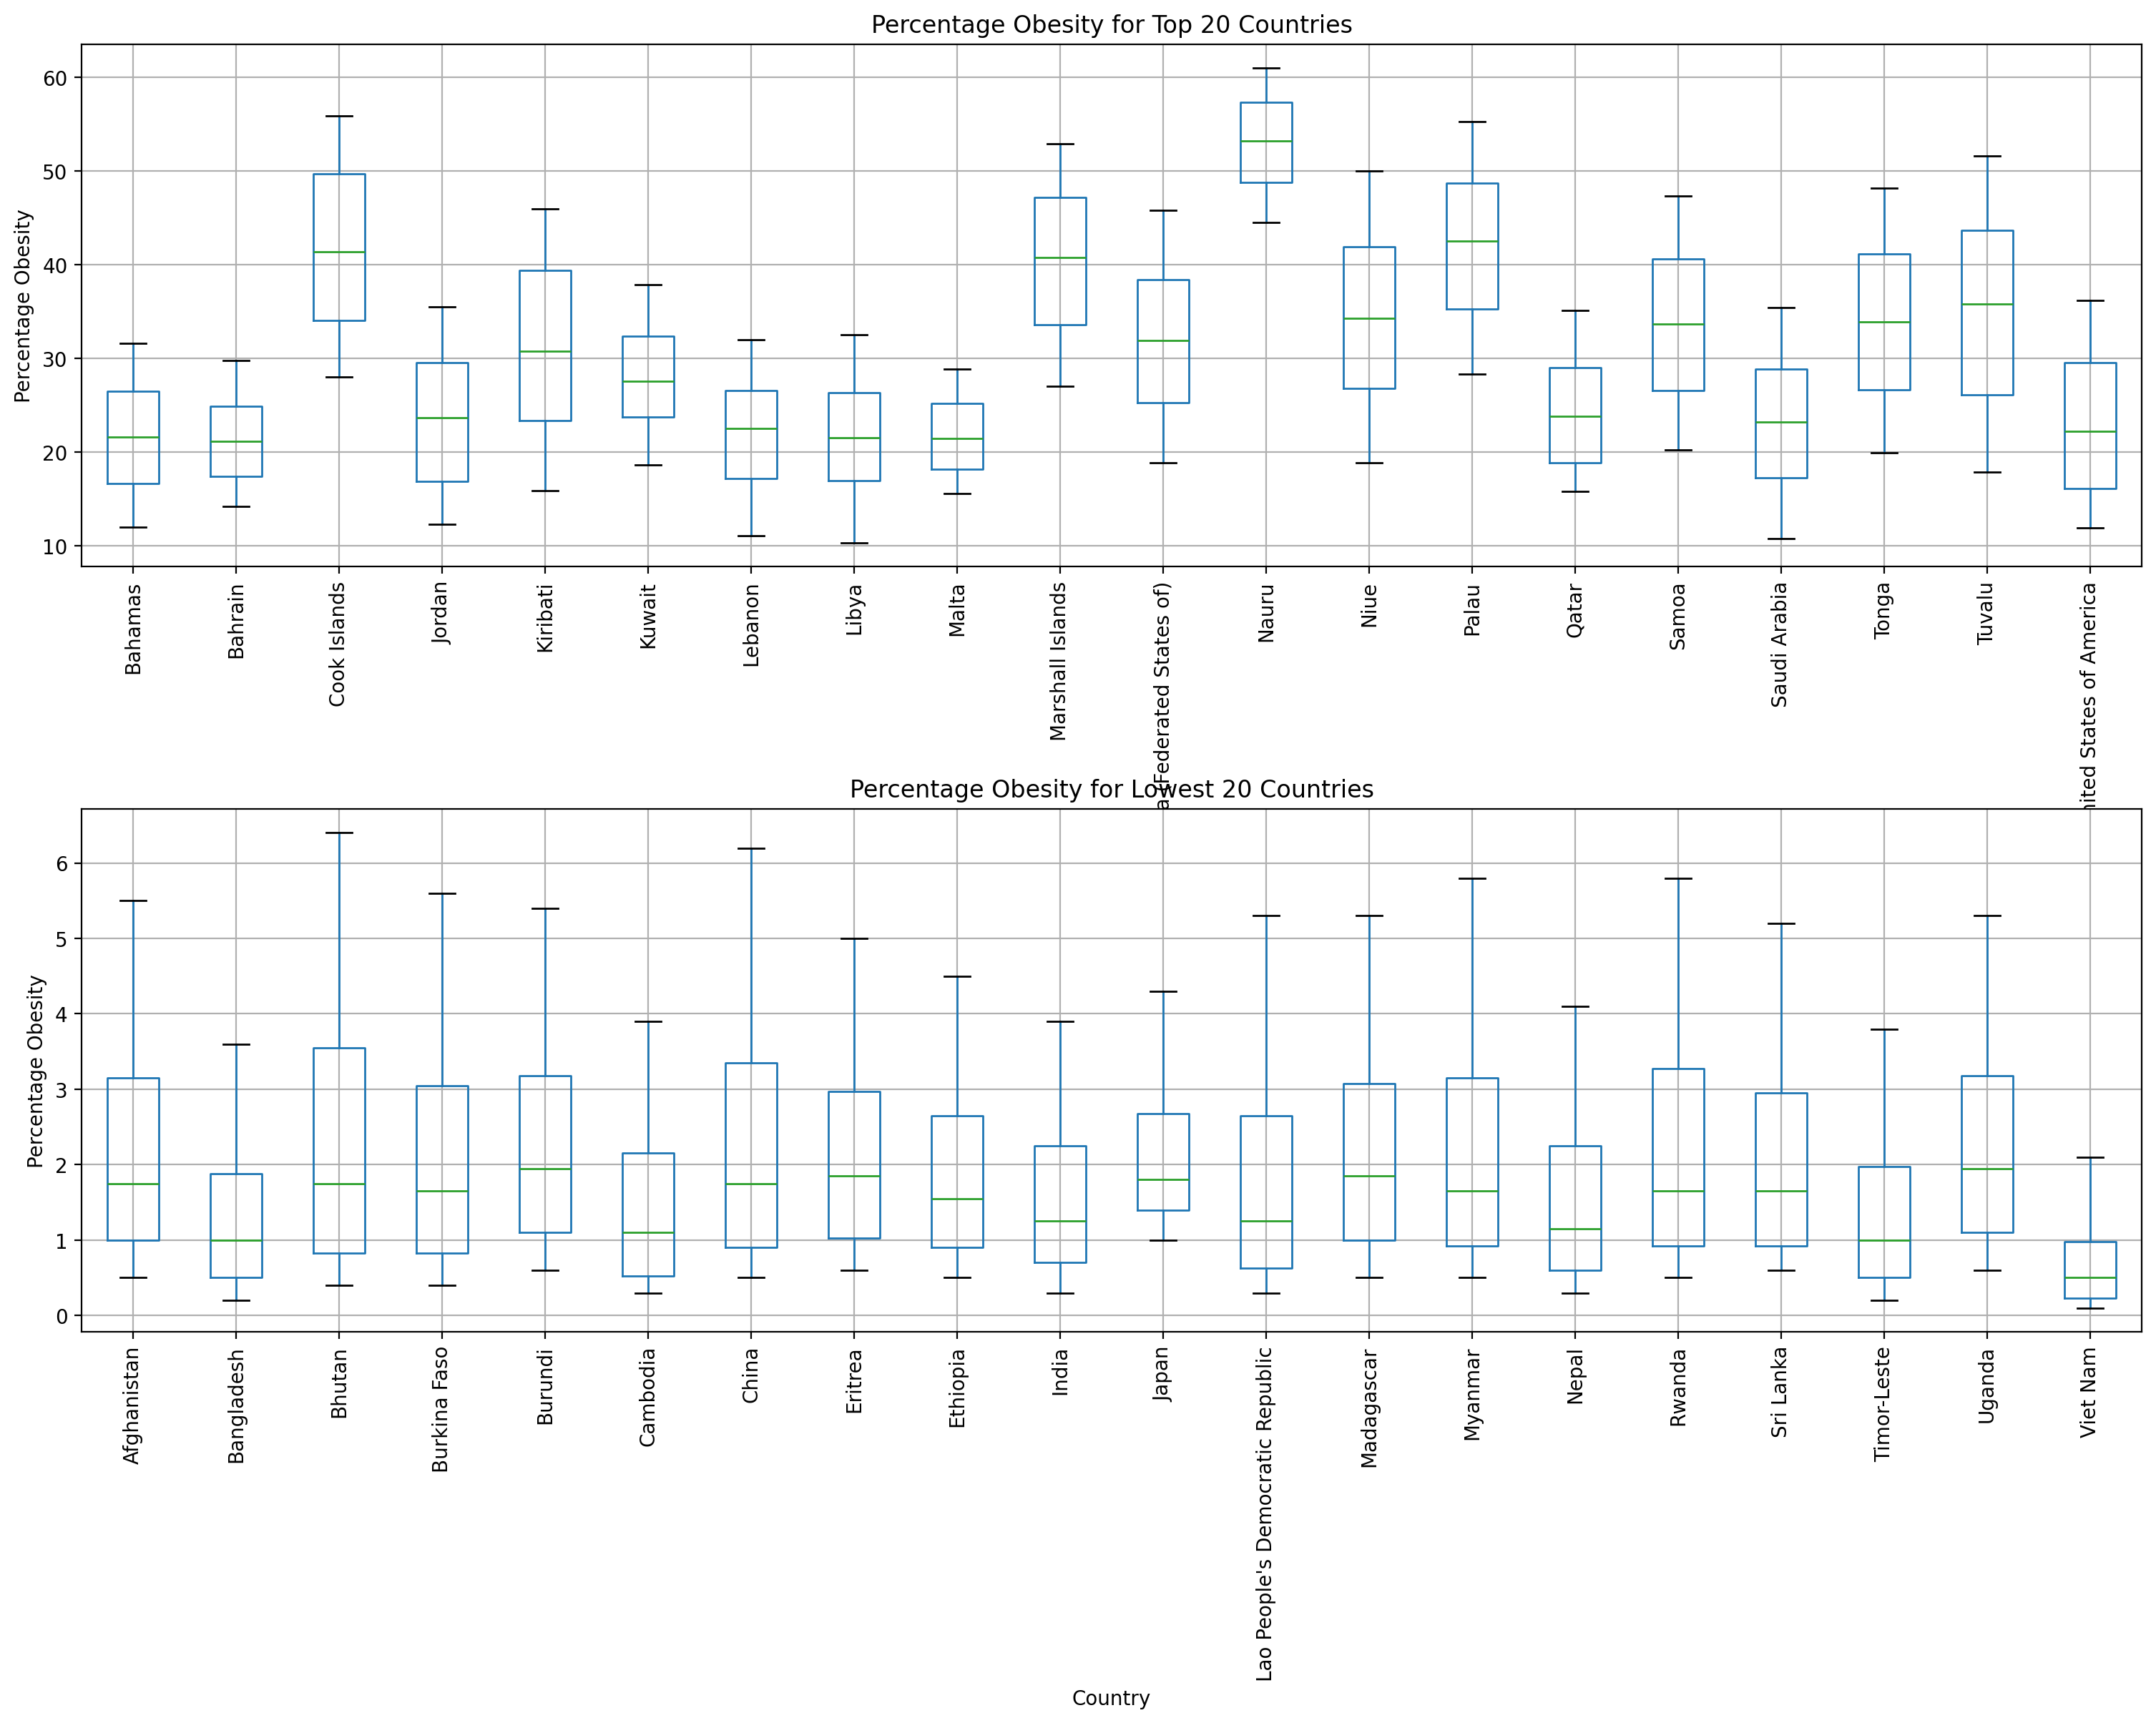
\includegraphics[scale=0.4]{images/du_obesity_pe_ob_cou_t_l_20}
                \caption{Percentages of obesity, 20 top countries at the top, 20 lowest a the button.}
                \label{fig:du-obesity-per-obe-countries-top-lw-20}
            \end{figure}

            Key takeaways from the boxplots include:

            \begin{itemize}
                \item \textbf{Top Countries:} Nauru, Cook Islands, Marshall Islands, and Palau are countries that feature prominently for having the highest obesity rates among the top 20 countries.

                \item \textbf{Bottom Countries:} On the opposite end, Vietnam and Bangladesh are among the countries with the lowest rates of obesity.

                \item \textbf{Time Frame:} The data encapsulates the years between 1975 and 2016, offering a broad historical perspective on obesity trends.
            \end{itemize}

            The juxtaposition of these two boxplots reveals striking differences in obesity prevalence across countries. It underscores the urgent need for tailored public health interventions, taking into account the unique challenges faced by countries at both ends of the obesity spectrum.


%            \begin{figure}[H]
%                \centering
%                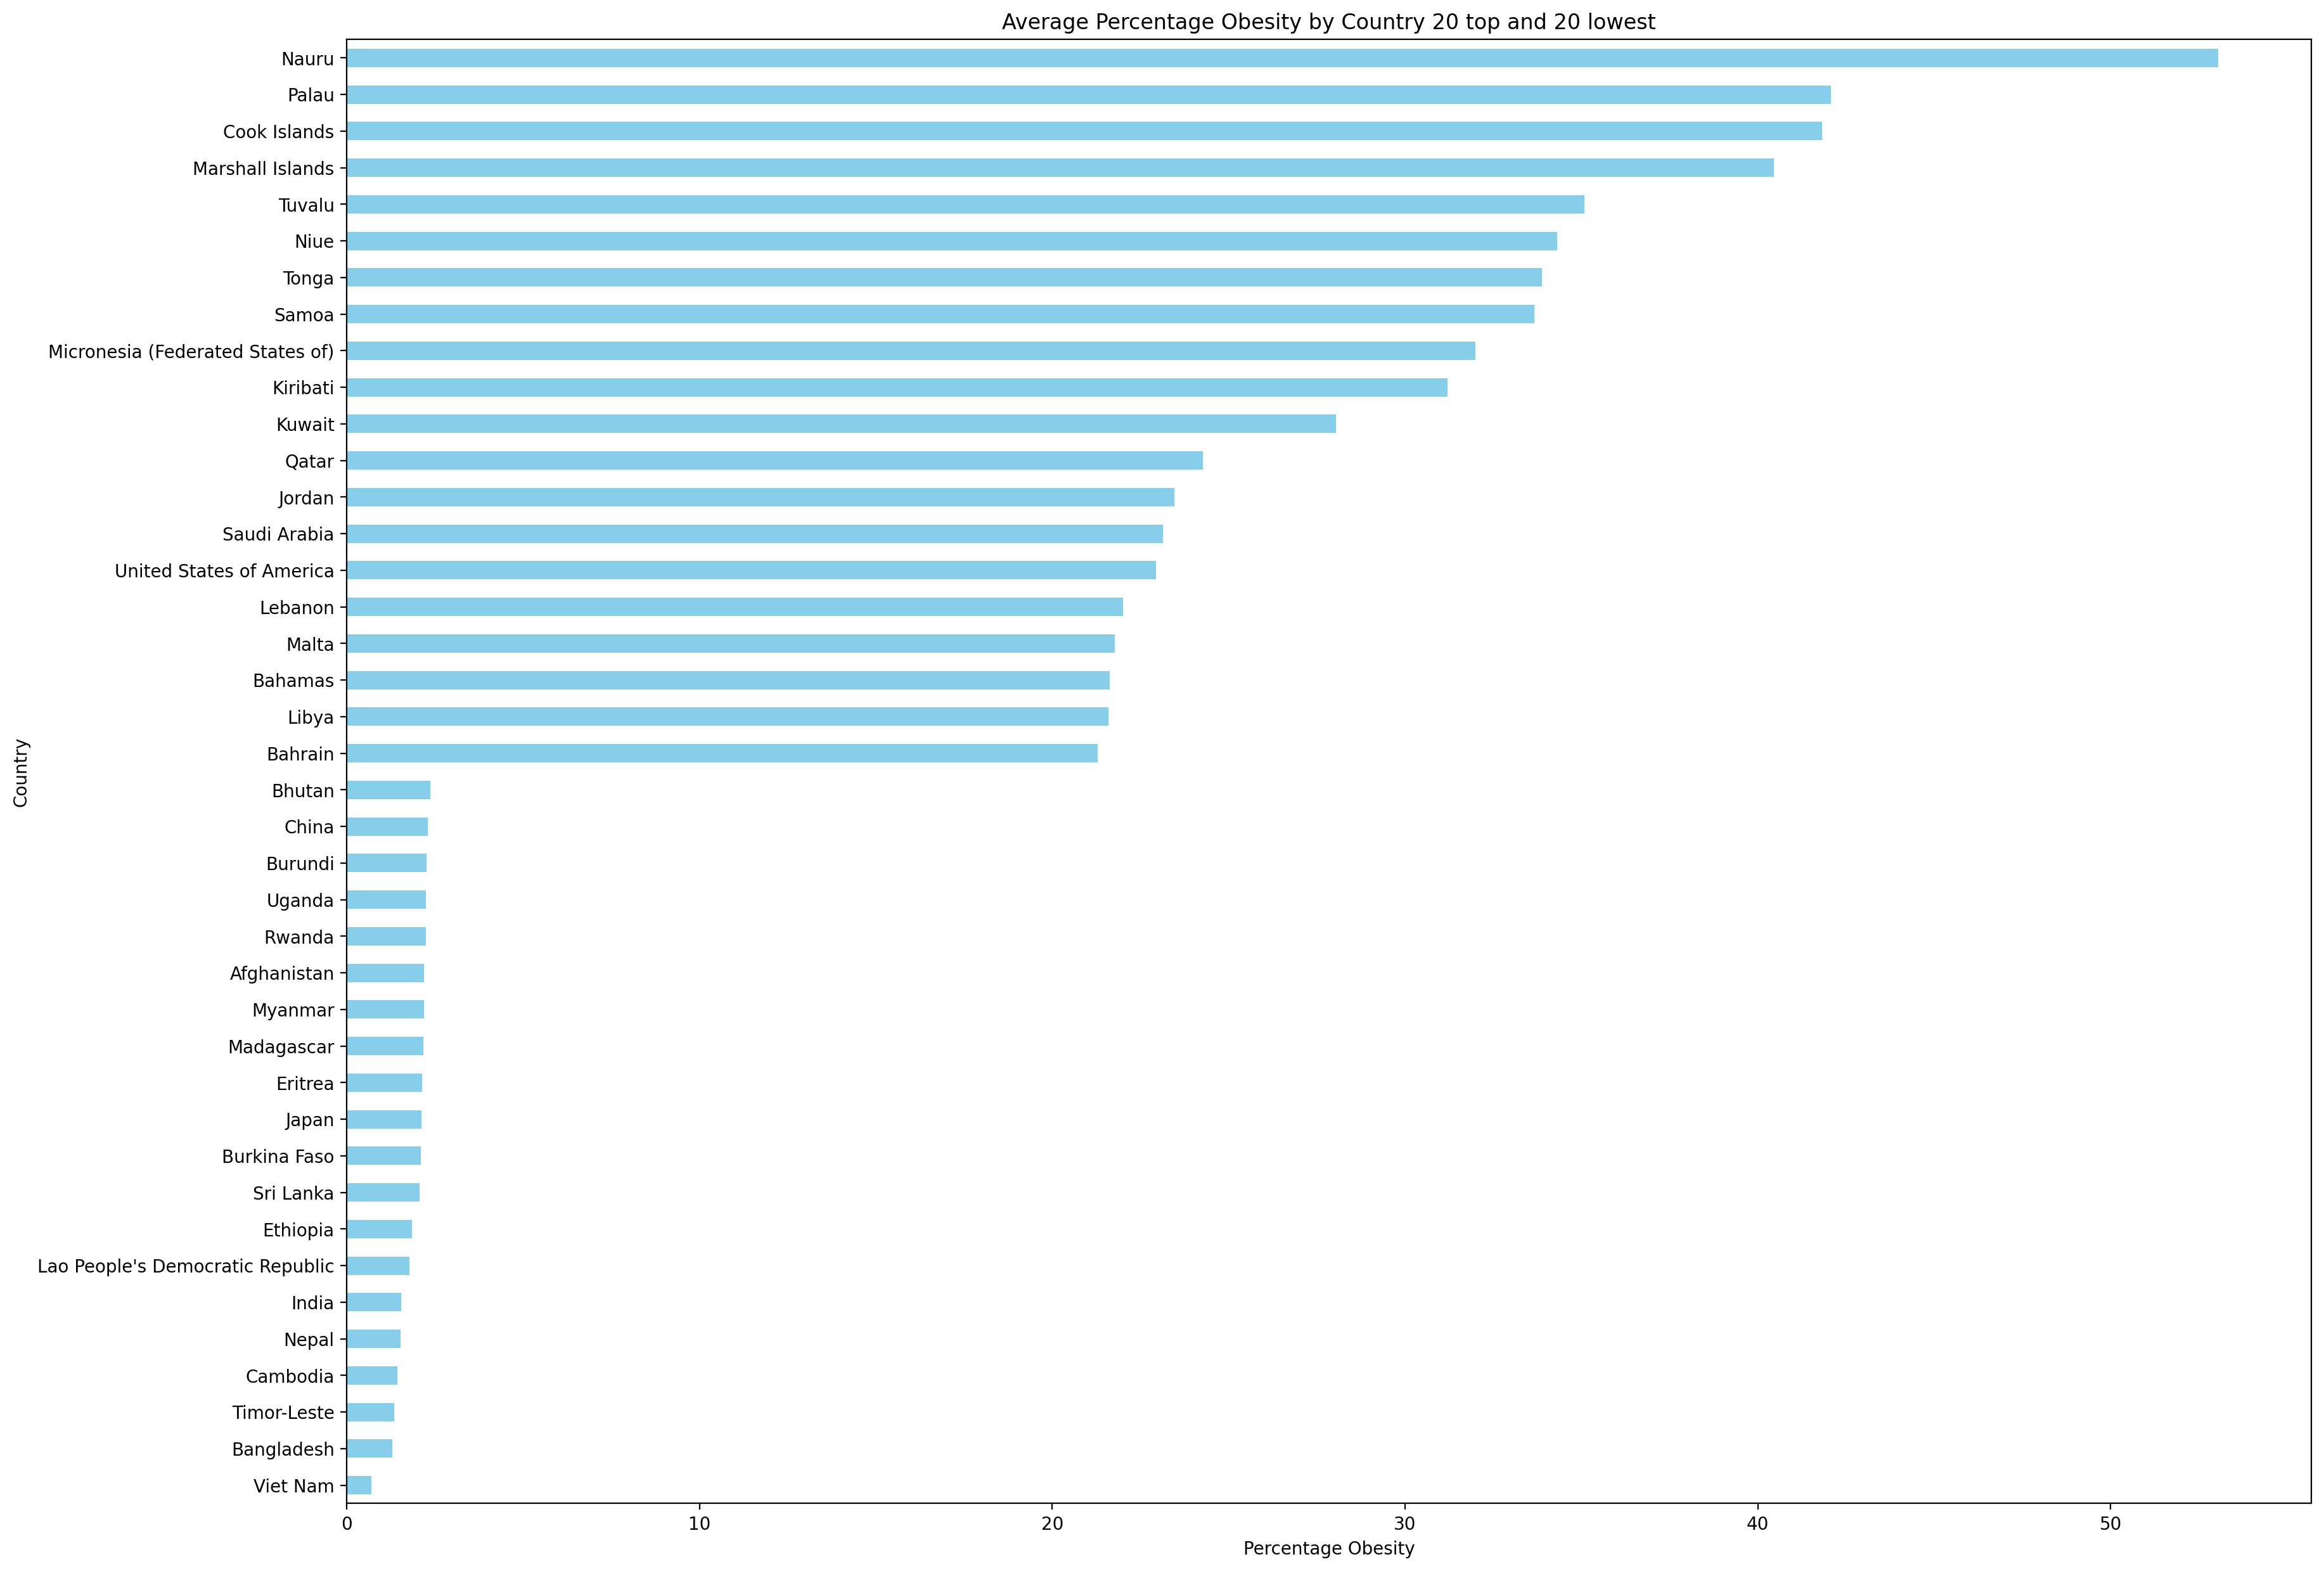
\includegraphics[scale=0.4]{images/du_obesity_pe_ob_cou_t_l_20_v2}
%                \caption{Percentages of obesity, 20 top and 20 lowest percentages by countries.}
%                \label{fig:du-obesity-per-obe-countries-top-ww-20-2}
%            \end{figure}

            \begin{figure}[H]
                \centering
                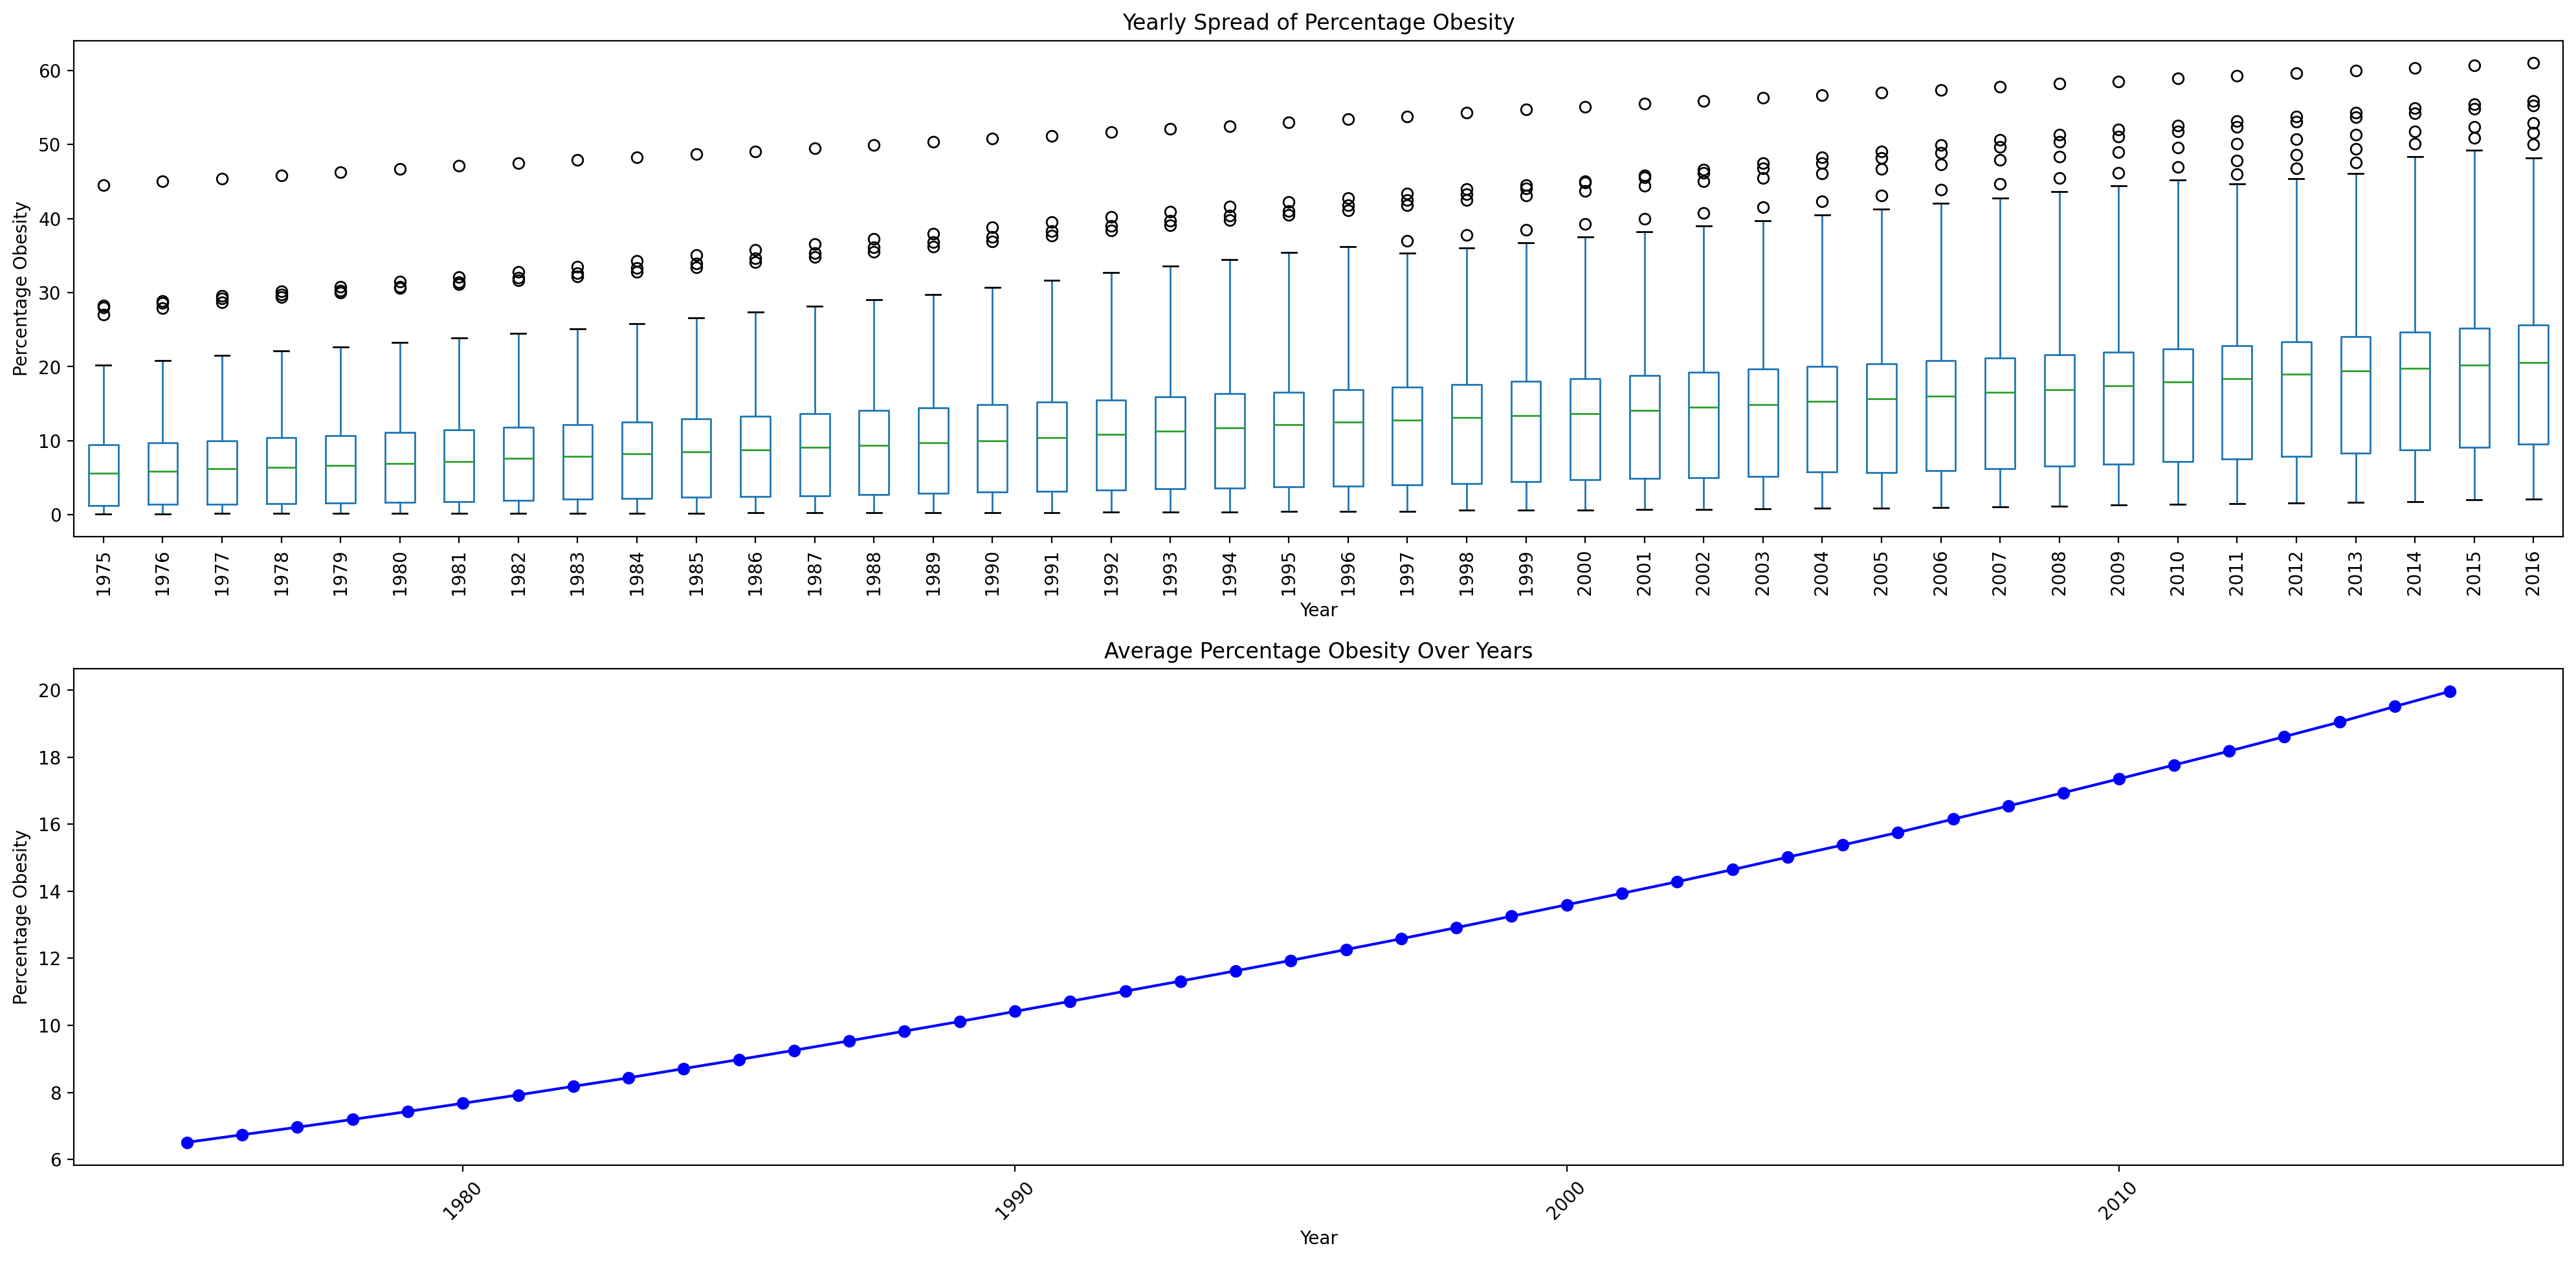
\includegraphics[scale=0.3]{images/du_obesity_pe_ob_y_trend}
                \caption{Trend of obesity percentages over years.}
                \label{fig:du-obesity-per-obe-trend-years}
            \end{figure}

            \figurename~\ref{fig:du-obesity-per-obe-trend-years} displays a boxplot illustrating the distribution of obesity percentages from the year 1975 to 2016.

            The plots reveals several key trends and characteristics:

            \begin{itemize}
                \item \textbf{Rising Means:} The mean obesity percentage has been steadily increasing over the years. It started at approximately 5\% in 1975 and has nearly tripled to around 20\% by 2016.

                \item \textbf{Increased Variability:} The size of the boxes, which represent the interquartile range (IQR), has grown over time. This indicates an increase in data variability. Despite this increased spread, most of the data still remain in the lower part of the box, below the mean.

                \item \textbf{Presence of Outliers:} The boxplot shows outliers that reach almost 60\%. These outliers are data points that are significantly higher than the other observations and indicate instances where the obesity rates are exceptionally high.
            \end{itemize}

            The boxplot suggests that although the general trend is an increase in obesity percentages, there are significant variances and outliers that should not be overlooked. These insights are crucial for designing effective public health interventions.

            \begin{figure}[H]
                \centering
                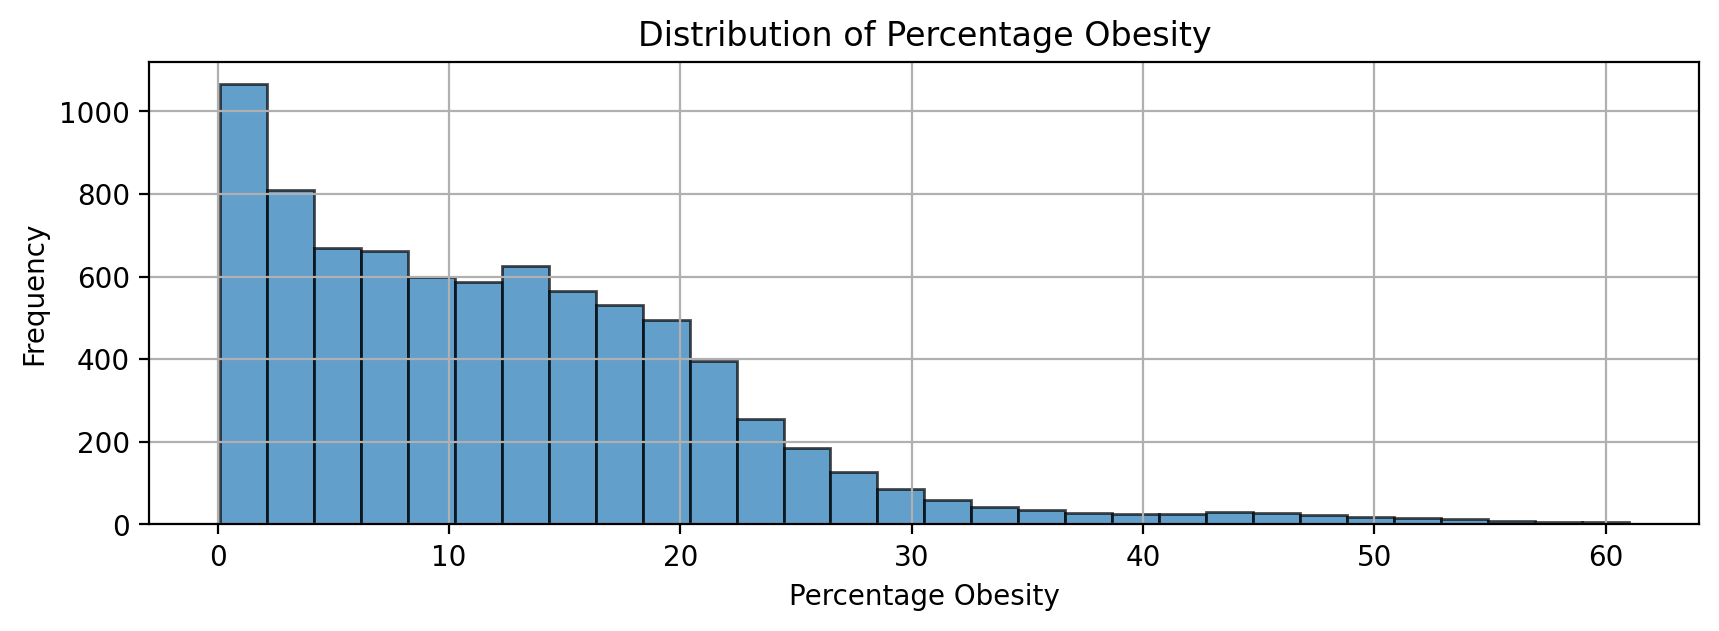
\includegraphics[scale=0.8]{images/du_obesity_pe_ob_freq}
                \caption{Distribution of obesity percentages.}
                \label{fig:du-obesity-per-obe-distribution}
            \end{figure}

            In the histogram of percentages of obesity (\figurename~\ref{fig:du-obesity-per-obe-distribution}), the majority of the observations are clustered in the lower percentage ranges, specifically between 0\% and 5\%. This area represents the peak of the distribution. As we move towards higher percentages, the frequency of observations decreases, forming a tail on the right side of the histogram.

            This right-skewed pattern suggests that while most regions or populations have low obesity rates, there are outliers with significantly higher percentages. These outliers are responsible for the long tail on the right side of the histogram.

            The right-skewed nature of this data may have implications for public health policies, as it indicates that while obesity is generally low, there are specific areas where it is unusually high.

            \subsubsection{Statistical Summary of {\dsObesity}}

                The \textit{\dsObesity} (\figurename~\ref{fig:du-obesity-summary}) provides several statistics, calculated over a range of years from 1975 to 2016. The dataset has a total of 24,650 entries, but some columns have missing data. Here's a simple breakdown of the statistical summary:

                \begin{itemize}
                        \item \textbf{Year:} The data spans from the year 1975 to 2016, with the average year being 1995.5. The dataset is uniformly spread, as indicated by a standard deviation of 12.12.

                        \item \textbf{Numeric:} This column seems to represent some obesity metric. The minimum value is 0.1 and the maximum is 63.3. The average value is around 12.42, with a standard deviation of 10.4, indicating a wide range of data points.

                        \item \textbf{Low:} This column has a minimum value of 0 and a maximum value of 55.6. The average is 9.21, and the data varies with a standard deviation of 8.85.

                        \item \textbf{High:} The data in this column ranges from 0.2 to 70.8, with an average value of 16.20. The standard deviation is 12, suggesting variability in the data.

                        \item \textbf{StdErr and StdDev:} These columns contain no data, as all entries are missing (NaN).
                \end{itemize}

                In summary, while the dataset provides a rich set of data points for some columns like \textit{Year}, \textit{Numeric}, \textit{Low}, and \textit{High}, it lacks any information in the \textit{StdErr} and \textit{StdDev} columns.


    \section{\dsMeat}

        \subsection{\duCollectInitialData}
            Our World In Data furnishes this database. Meat consumption is a reflection of living standards and dietary patterns. This indicator encompasses beef, pork, poultry, fish, and sheep, measured in kilograms per capita per year.
            \\
            \\
            The data originates from FAOSTAT (Food and Agriculture Organization of the United Nations), sourced from distinct datasets for each meat category.
            \\
            \\
            Accessing data through Our World In Data is convenient, offering options for full or selective downloads. The presentation choices include charts, maps, and tables, streamlining the analysis process.

        \subsection{\duDescribeTheData}
            \begin{figure}[H]
                \centering
                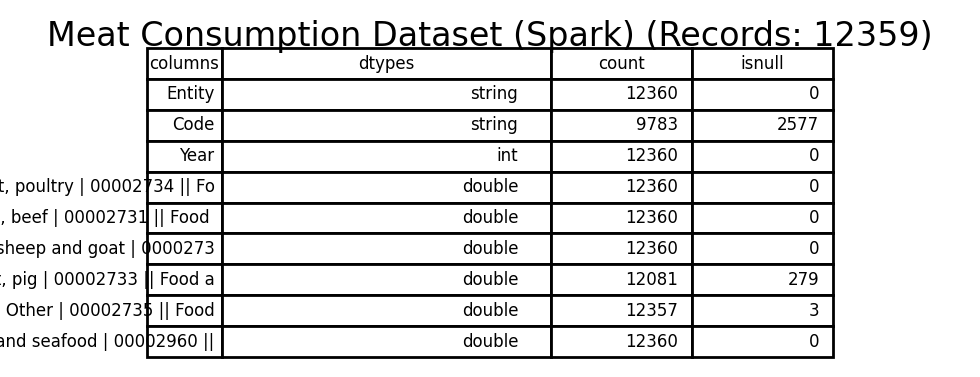
\includegraphics[scale=1.3]{images/du_meat_consumption_dataset}
                \caption{Contains the information of different sort of meat consumed by country and year.}
                \label{fig:du-meat-datasets}
            \end{figure}

            The \textit{\dsMeat} (\figurename~\ref{fig:du-meat-datasets}) comprises 12,360 entries and is divided into 9 columns.

            \textbf{Text-based Columns:}
            \begin{enumerate}
                \item \textit{Entity}: Describes the geographical or organizational entity and is complete with no missing values.
                \item \textit{Code}: Appears to be some kind of identifier code but has 2,577 missing entries.
            \end{enumerate}

            \textbf{Numerical Columns:}
            \begin{enumerate}
                \item \textit{Year}: An integer column that indicates the year of data collection, and it has no missing values.
                \item \textit{Meat, poultry}: A float column that measures the availability of poultry meat in kilograms per year per capita. It has no missing values.
                \item \textit{Meat, beef}: Another float column that measures beef availability in kilograms per year per capita, also with no missing entries.
                \item \textit{Meat, sheep and goat}: A float column detailing the availability of sheep and goat meat, with no missing values.
                \item \textit{Meat, pig}: This float column measures the availability of pig meat but has 279 missing entries.
                \item \textit{Meat, Other}: Another float column that covers other types of meat, with only 3 missing values.
                \item \textit{Fish and seafood}: A float column that measures the availability of fish and seafood, with no missing values.
            \end{enumerate}

            In summary, the dataset is largely complete, with most columns having no missing values. However, the \textit{Code} column has a significant number of missing entries, and the \textit{Meat, pig} column has some missing values as well.

        \subsection{\duExploreTheData}
            \begin{figure}[H]
                \centering
                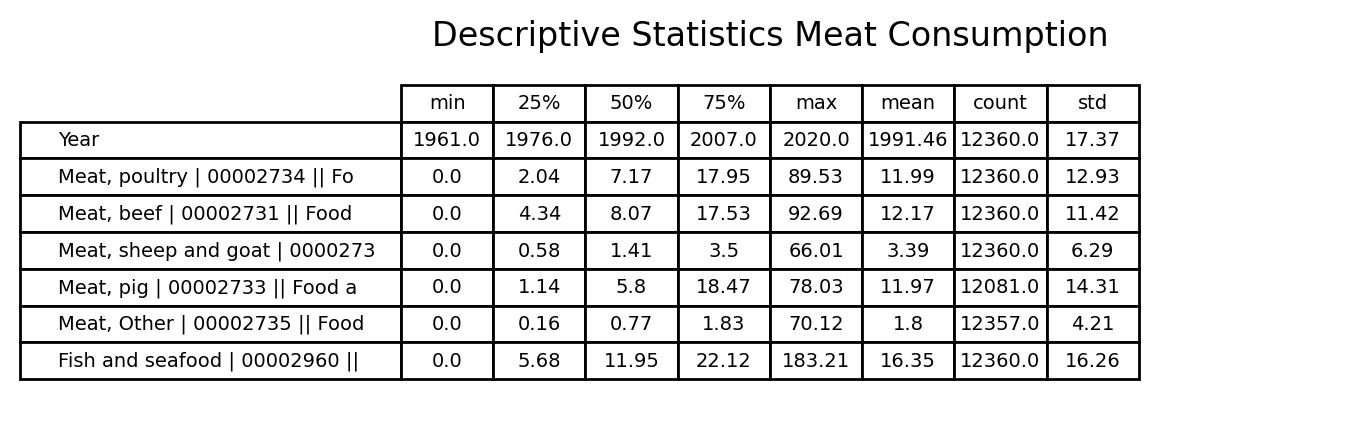
\includegraphics[scale=1]{images/du_meat_consumption_summary}
                \caption{}
                \label{fig:du-meat-summary}
            \end{figure}

            \subsubsection{Statistical Summary of {\dsMeat}}

                The {\dsMeat} (\figurename~\ref{fig:du-meat-summary}) offers a wealth of information captured over several years, specifically from 1961 to the most recent data. The dataset contains a total of 12,360 entries. Here is a straightforward summary of key statistics for each column:


                \begin{itemize}
                        \item \textbf{Year:} The data spans from 1961 to 2020, with an average year of around 1991. A standard deviation of 17.37 suggests a uniform distribution of data over the years.

                        \item \textbf{Meat, poultry:} The consumption ranges from 0 to 89.53 kilograms per person per year. The average is about 11.99 kilograms with a standard deviation of 12.93, showing wide variability.

                        \item \textbf{Meat, beef:} The dataset has a minimum value of 0 and a maximum of 92.69 kilograms per person per year. The average is 12.17 kilograms with a standard deviation of 11.42.

                        \item \textbf{Meat, sheep and goat:} The average consumption is around 3.39 kilograms per person per year. With a standard deviation of 6.29, this column shows significant variations across data points.

                        \item \textbf{Meat, pig:} The average is approximately 11.97 kilograms per person per year, and the standard deviation is 14.31. This column has 279 missing entries.

                        \item \textbf{Meat, Other:} Average consumption stands at 1.80 kilograms per person per year. The standard deviation of 4.21 indicates a wide range of data points.

                        \item \textbf{Fish and seafood:} On average, 16.35 kilograms are consumed per person per year. The standard deviation is 16.26, suggesting a wide range of consumption rates.
                \end{itemize}

                In summary, the dataset is mostly complete, providing a diverse set of measurements across different types of meat and seafood. However, the \textit{Meat, pig} column has some missing values.


    \section{\dsHappiness}

        \subsection{\duCollectInitialData}
            The World Happiness Report 2023 encompasses a range of indices addressing diverse facets of human existence. These indices draw upon not only subjective metrics but also psychological perceptions held by each population about their respective countries.
            \\
            \\
            This dataset amalgamates information from various sources to enhance the ultimate score, leveraging this integration to construct the foundational dataset from which the World Happiness Report is generated. Accessing this database is straightforward and user-friendly.

        \subsection{\duDescribeTheData}
            \begin{figure}[H]
                \centering
                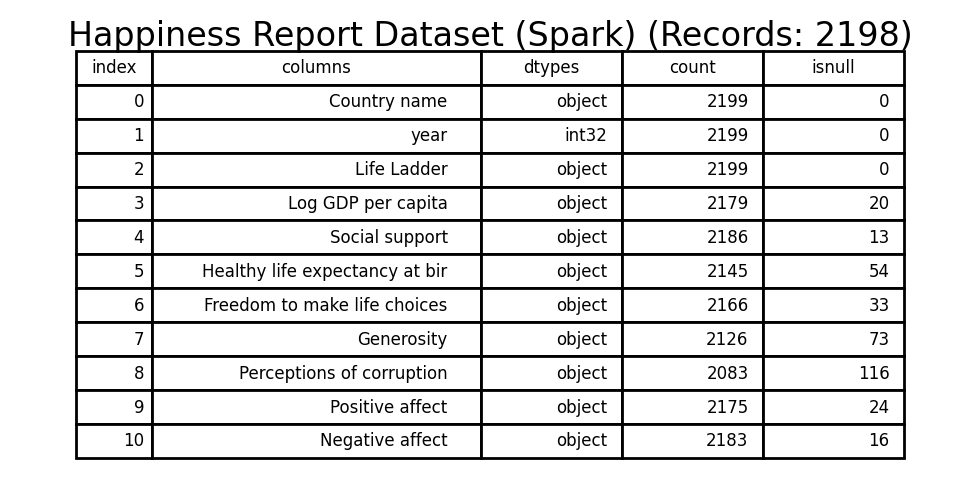
\includegraphics[scale=1.3]{images/du_happiness_dataset}
                \caption{Contains the information of index of happiness and others metrics by country and year.}
                \label{fig:du-happiness-datasets}
            \end{figure}

            The \textit{\dsHappiness}(\figurename~\ref{fig:du-happiness-datasets}) contains 2,199 entries, organized into 11 columns.

            \textbf{Text-based Column:}
            \begin{enumerate}
                \item \textit{Country name}: Describes the name of the country and is complete with no missing values.
            \end{enumerate}

            \textbf{Numerical Columns:}
            \begin{enumerate}
                \item \textit{year}: An integer column indicating the year the data was collected, with no missing entries.
                \item \textit{Life Ladder}: A float column that presumably measures the happiness index. It has no missing values.
                \item \textit{Log GDP per capita}: A float column representing the logarithm of the GDP per capita, with 20 missing entries.
                \item \textit{Social support}: Float column representing social support metrics, with 13 missing values.
                \item \textit{Healthy life expectancy at birth}: Float column with 54 missing entries.
                \item \textit{Freedom to make life choices}: Float column with 33 missing values.
                \item \textit{Generosity}: A float column measuring generosity, with 73 missing entries.
                \item \textit{Perceptions of corruption}: Float column with 116 missing values.
                \item \textit{Positive affect}: Float column representing positive emotions, with 24 missing entries.
                \item \textit{Negative affect}: Float column representing negative emotions, with 16 missing entries.
            \end{enumerate}

            In summary, while the \textit{Country name} and \textit{year} columns are complete, several of the float columns have missing values, with the \textit{Perceptions of corruption} column having the highest number of missing entries.

            \subsubsection{Fields explanation}

                \begin{itemize}

                        \item \textbf{Happiness Score (Ladder):} This metric gauges individuals' subjective well-being using data from the Gallup World Poll between 2005 and 2022. Respondents assign life evaluations on a scale from 0 to 10.

                        \item \textbf{GDP Per Capita (PPP):} This feature presents economic data, accounting for purchasing power parity in constant 2017 international dollars. It combines information from the World Development Indicators (WDI) and the Penn World Table 10.01, which supplements data for certain nations.

                        \item \textbf{Healthy Life Expectancy (HLE):} Calculated from the World Health Organization's Global Health Observatory, this indicator predicts life expectancy based on health data. Interpolation and extrapolation are applied to align the range with the dataset's timeline (2005-2021).

                        \item \textbf{Social Support:} This measure captures the availability of assistance during challenging times. Respondents answer a binary question in the Gallup World Poll. Answer to the question ``If you were in trouble, do you have relatives or friends you can count on to help you whenever you need them, or not?''

                        \item \textbf{Freedom to Make Life Choices:} Reflecting personal satisfaction with individual freedom, this metric originates from GWP responses. Answer to the question ``Are you satisfied or dissatisfied with your freedom to choose what you do with your life?''

                        \item \textbf{Generosity:} Derived as a residual value from the relationship between charitable contributions and GDP per capita. Answer to the question ``Have you donated money to a charity in the past month?''

                        \item \textbf{Corruption Perception:} Extracted from GWP responses about government and business corruption, the overall perception is obtained by averaging 0-or-1 responses.

                        \item \textbf{Positive Affect:} This figure represents the average of affirmative responses to queries about positive emotions like laughter, enjoyment, and engaging activities during specific Gallup World Poll waves. Based on the questions ``Did you smile or laugh a lot yesterday?'', and ``Did you experience the following feelings during A LOT OF THE DAY yesterday? How about Enjoyment?'', ``Did you learn or do something interesting yesterday?''

                        \item \textbf{Negative Affect:} This index calculates the average of negative emotions such as worry, sadness, and anger reported in particular Gallup World Poll waves. Based on the questions ``Did you experience the following feelings during A LOT OF THE DAY yesterday? How about Worry?'', ``Did you experience the following feelings during A LOT OF THE DAY yesterday? How about Sadness?'', and ``Did you experience the following feelings during A LOT OF THE DAY yesterday? How about Anger?''

                \end{itemize}

        \subsection{\duExploreTheData}
            \begin{figure}[H]
                \centering
                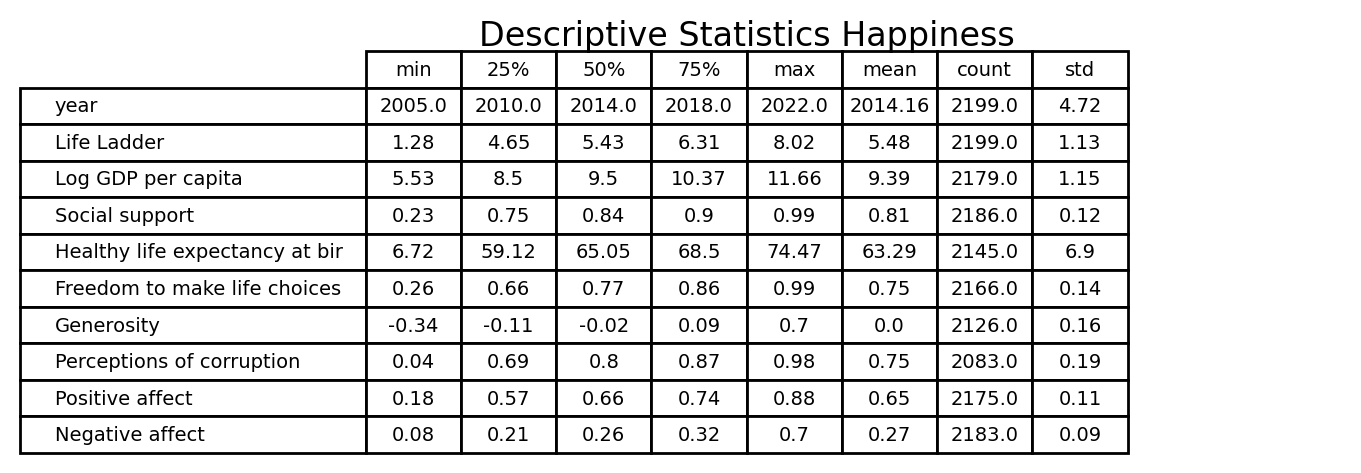
\includegraphics[scale=1]{images/du_happiness_summary}
                \caption{}
                \label{fig:du-happiness-summary}
            \end{figure}

            \subsubsection{Statistical Summary of \dsHappiness}

                The \textit{\dsHappiness}(\figurename~\ref{fig:du-happiness-summary}) offers a thorough exploration into various factors contributing to happiness, spanning from the year 2005 to 2022. The dataset consists of 2,199 entries, although some columns have a few missing values. Here's a straightforward explanation of its key statistics:

                \begin{itemize}
                        \item \textbf{Year:} The dataset ranges from 2005 to 2022, with an average year around 2014. A standard deviation of 4.72 suggests a balanced distribution of data across the years.

                        \item \textbf{Life Ladder:} This score ranges from 1.28 to 8.02, with an average of approximately 5.48. The standard deviation of 1.13 shows moderate variability in happiness scores.

                        \item \textbf{Log GDP per capita:} The logarithm of GDP per capita ranges from 5.53 to 11.66, averaging at 9.39. This column has a standard deviation of 1.15 and 20 missing entries.

                        \item \textbf{Social support:} The values range from 0.23 to 0.99, with an average of 0.81 and a standard deviation of 0.12.

                        \item \textbf{Healthy life expectancy at birth:} Averages at 63.29 years with a standard deviation of 6.90, indicating a broad range in life expectancy.

                        \item \textbf{Freedom to make life choices:} Average freedom score stands at 0.75, with a standard deviation of 0.14, indicating relatively consistent freedom levels.

                        \item \textbf{Generosity:} Ranges from -0.34 to 0.70, averaging near zero, with a standard deviation of 0.16.

                        \item \textbf{Perceptions of corruption:} The average perception score is 0.75, with a standard deviation of 0.19. This column has 116 missing entries.

                        \item \textbf{Positive affect:} Averages at 0.65 with a standard deviation of 0.11, indicating a moderate level of positive emotional experiences.

                        \item \textbf{Negative affect:} Averages at 0.27 with a standard deviation of 0.09, indicating a low level of negative emotional experiences.
                \end{itemize}

                In summary, the dataset provides a comprehensive view on various factors affecting happiness levels. However, some columns have missing values, which should be taken into account when interpreting the data.


    \section{\dsAlcohol}

        \subsection{\duCollectInitialData}
            Leveraging data from Our World In Data offers a convenient advantage, offering the choice between comprehensive or specific data downloads. The presentation options include charts, maps, and tables, simplifying the process of conducting analysis.

        \subsection{\duDescribeTheData}
            \begin{figure}[H]
                \centering
                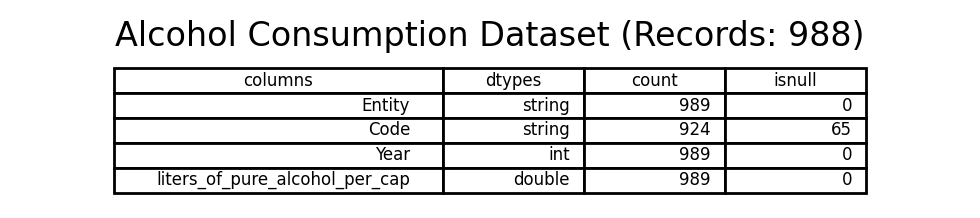
\includegraphics[scale=1.3]{images/du_alcohol_consumption_dataset}
                \caption{Contains the information of amount of pure alcohols in liters by country and year.}
                \label{fig:du-alcohol-datasets}
            \end{figure}

            The \textit{\dsAlcohol} (\figurename~\ref{fig:du-alcohol-datasets}) comprises 989 entries and is structured into 4 columns.

            \textbf{Text-based Columns:}
            \begin{enumerate}
                \item \textit{Entity}: Describes the geographical or organizational entity, and it is complete with no missing values.
                \item \textit{Code}: Functions as a code or identifier for the entity but has 65 missing entries.
            \end{enumerate}

            \textbf{Numerical Columns:}
            \begin{enumerate}
                \item \textit{Year}: An integer column indicating the year for which the data was collected. It has no missing values.
                \item \textit{liters\_of\_pure\_alcohol\_per\_capita}: This float column measures the consumption of pure alcohol per capita in liters. It is also complete with no missing entries.
            \end{enumerate}

            In summary, the dataset is nearly complete, with the only column having missing data being \textit{Code}, which has 65 missing entries.

        \subsection{\duExploreTheData}

            \figurename~\ref{fig:du-alcohol-countries-top-lw-20} displays two vertically stacked boxplots that capture the liters of pure alcohol consumption per capita. The top boxplot represents the data for the countries with the highest levels of alcohol consumption, while the bottom boxplot exhibits the same metric for the countries with the lowest levels. These measurements span the years 2000 to 2018.

            \begin{figure}[H]
                \centering
                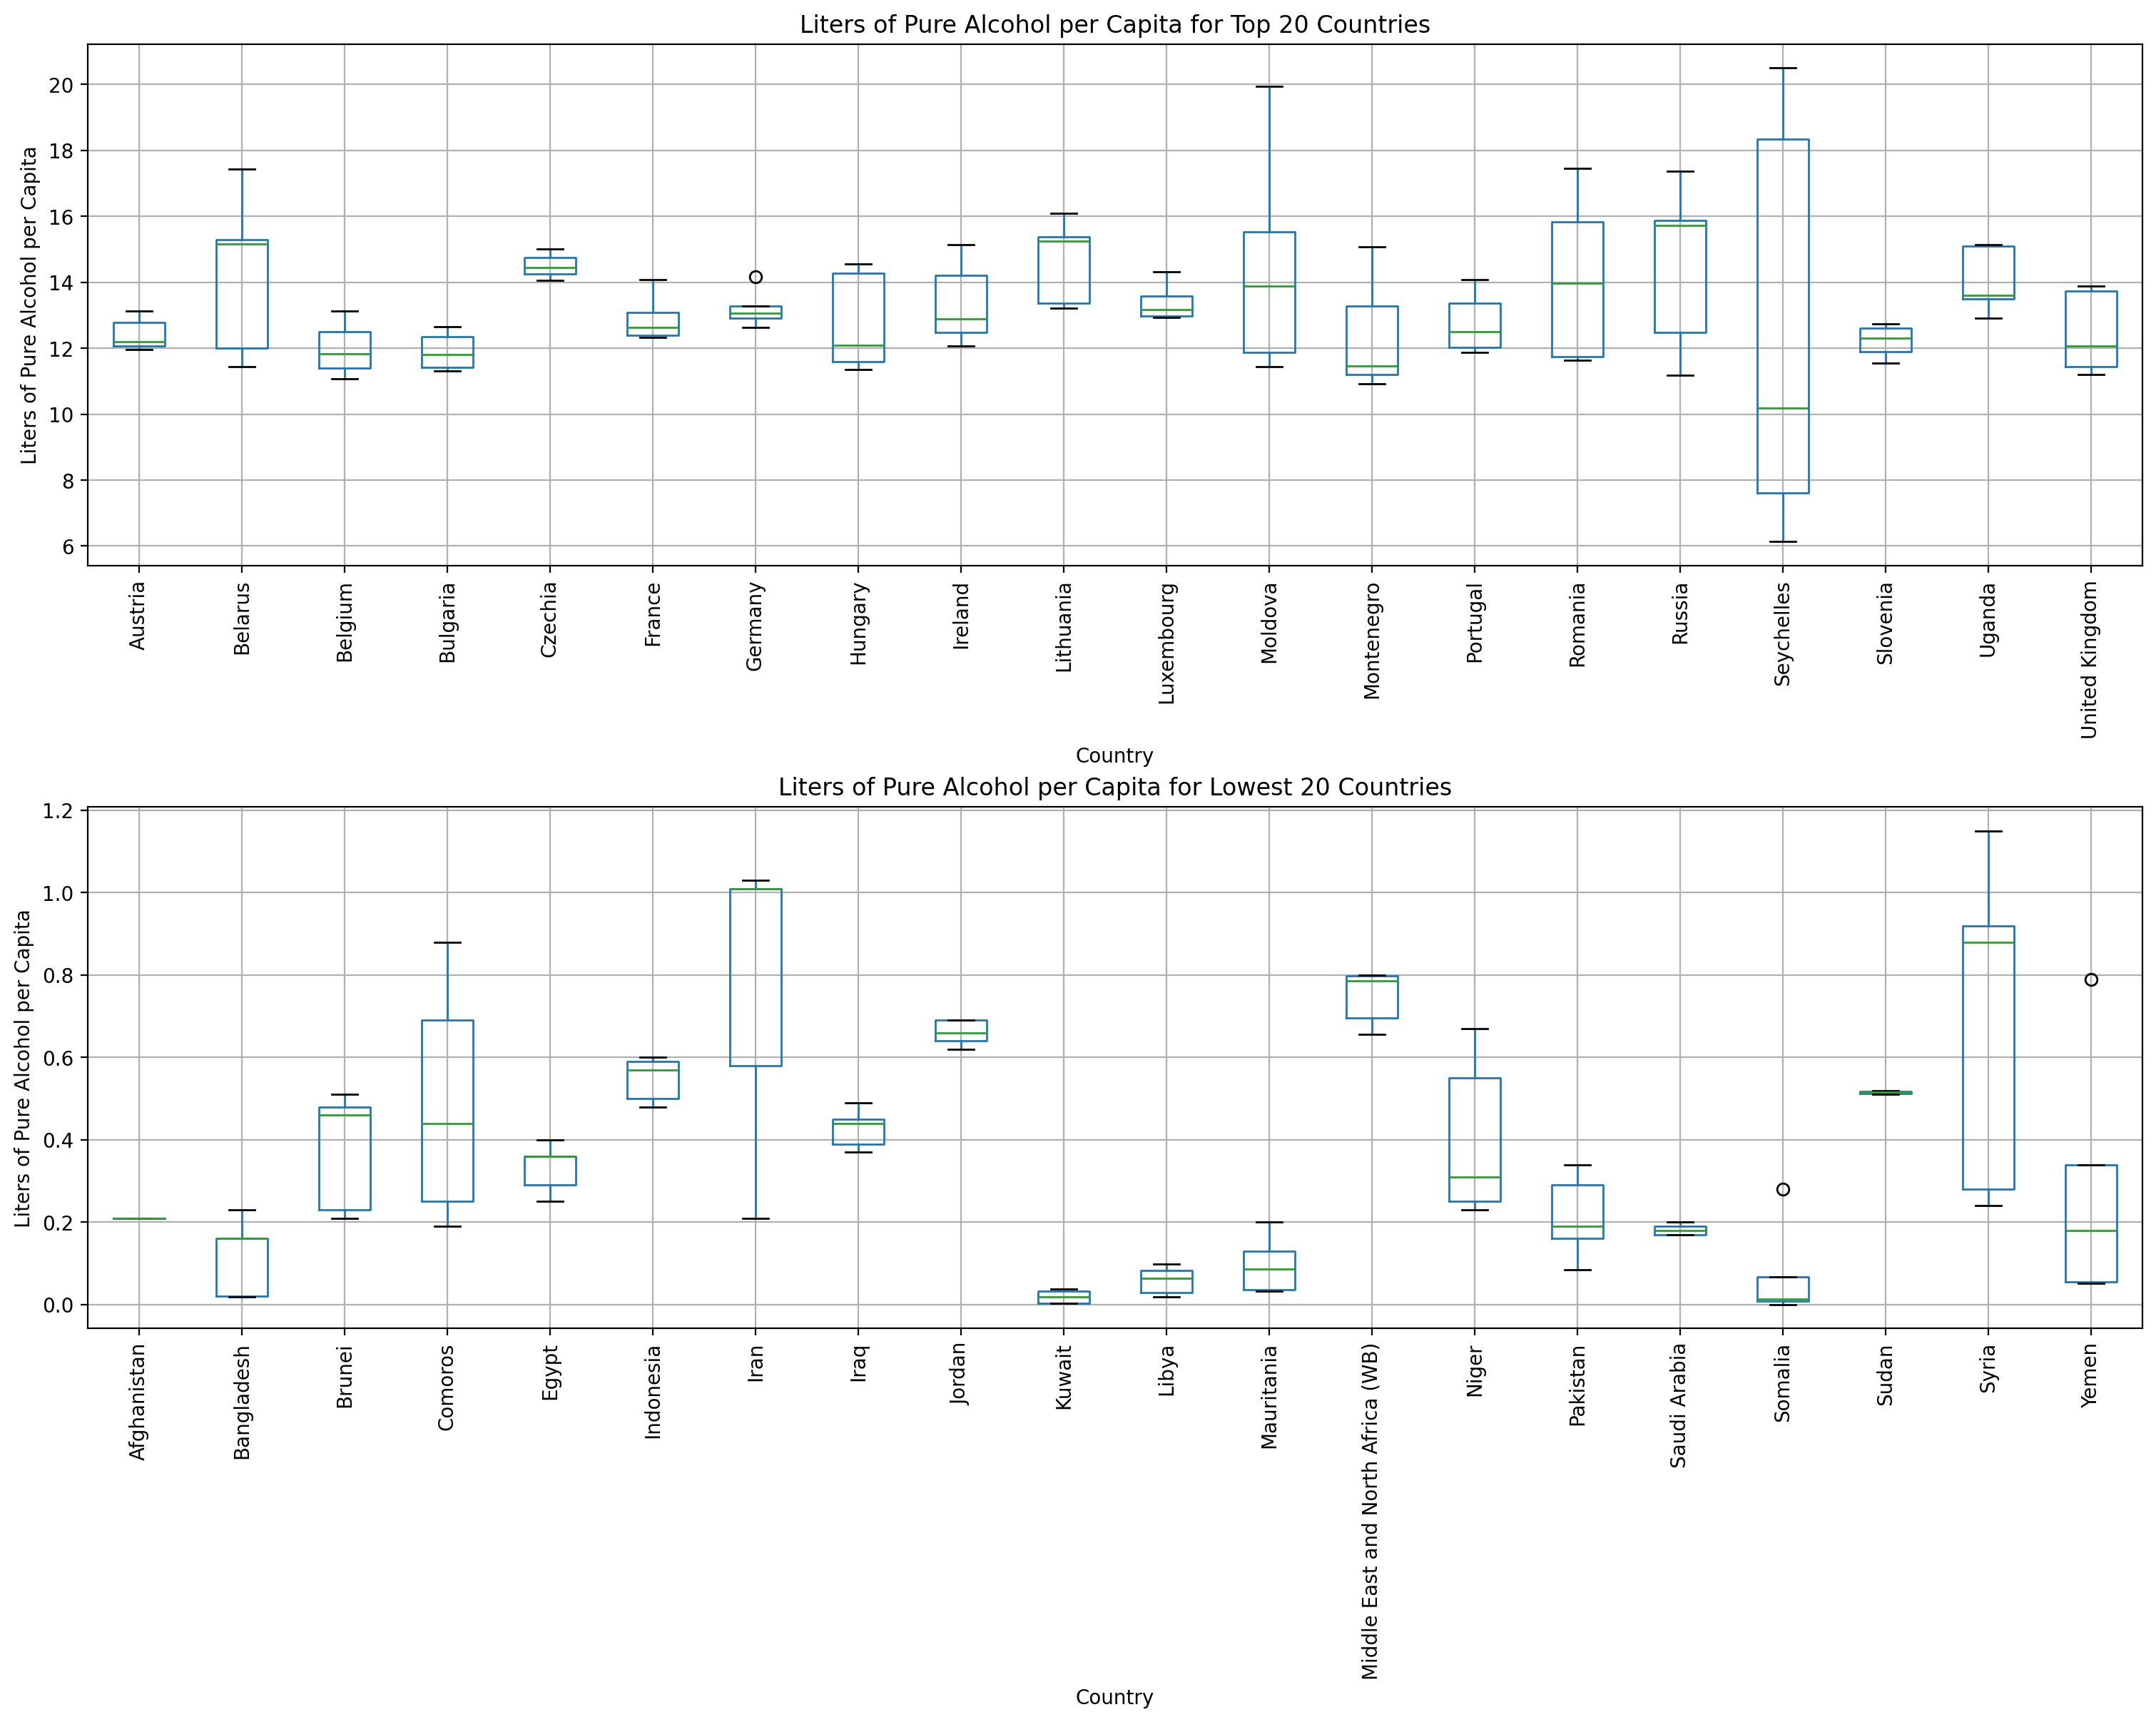
\includegraphics[scale=0.4]{images/du_alcohol_li_of_pu_al_pe_ca_cou_t_l_20}
                \caption{Liters of pure alcohol consumption per capita, 20 top countries at the top, 20 lowest a the button.}
                \label{fig:du-alcohol-countries-top-lw-20}
            \end{figure}

            Key highlights from the boxplots are as follows:

            \begin{itemize}
                \item \textbf{Top Consuming Countries:} Belarus and Moldova are notably among the countries with the highest levels of alcohol consumption.

                \item \textbf{Lowest Consuming Countries:} In contrast, Somalia and Kuwait are among those with the lowest alcohol consumption rates.

                \item \textbf{Few Outliers:} There are relatively few outliers in the data, suggesting that consumption levels within each group are fairly consistent.

                \item \textbf{Time Period:} The data represents a period from the year 2000 to 2018, offering an in-depth look into alcohol consumption trends over nearly two decades.
            \end{itemize}

            The side-by-side presentation of these boxplots illustrates stark differences in alcohol consumption habits across different countries. The data indicates the necessity for country-specific approaches to address issues related to alcohol consumption.

%            \begin{figure}[H]
%                \centering
%                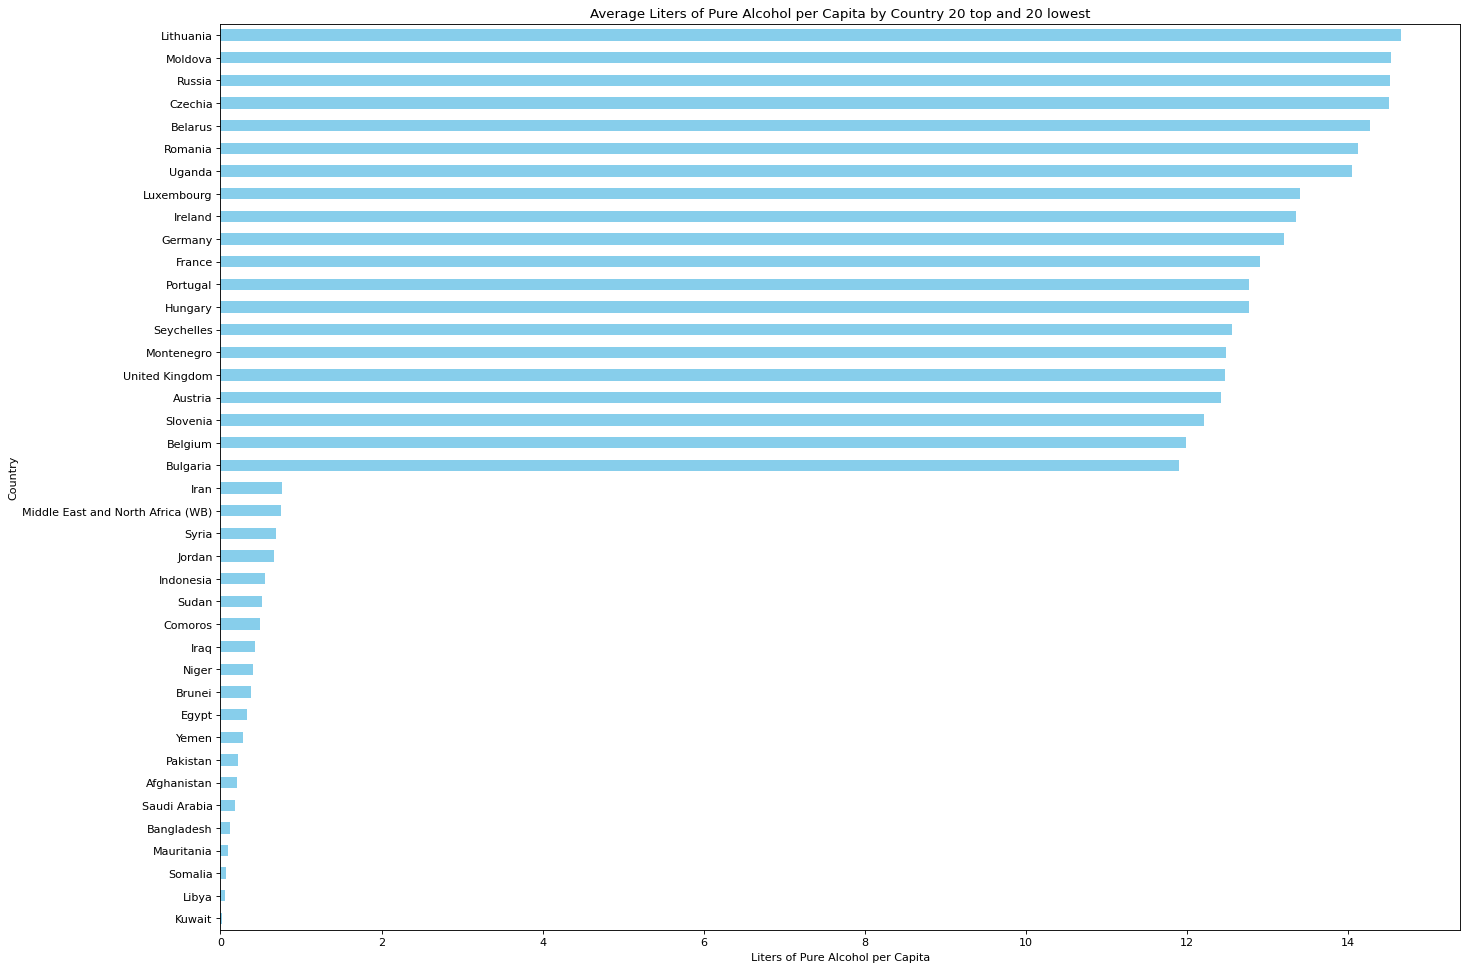
\includegraphics[scale=0.3]{images/du_alcohol_li_of_pu_al_pe_ca_cou_t_l_20_v2}
%                \caption{Liters of pure alcohol consumption per capita, 20 top and 20 lowest percentages by countries.}
%                \label{fig:du-alcohol-countries-top-ww-20-2}
%            \end{figure}

            \figurename~\ref{fig:du-alcohol-trend-years} shows a boxplot that outlines the distribution of liters of pure alcohol consumed per capita over a period of 8 years.

            \begin{figure}[H]
                \centering
                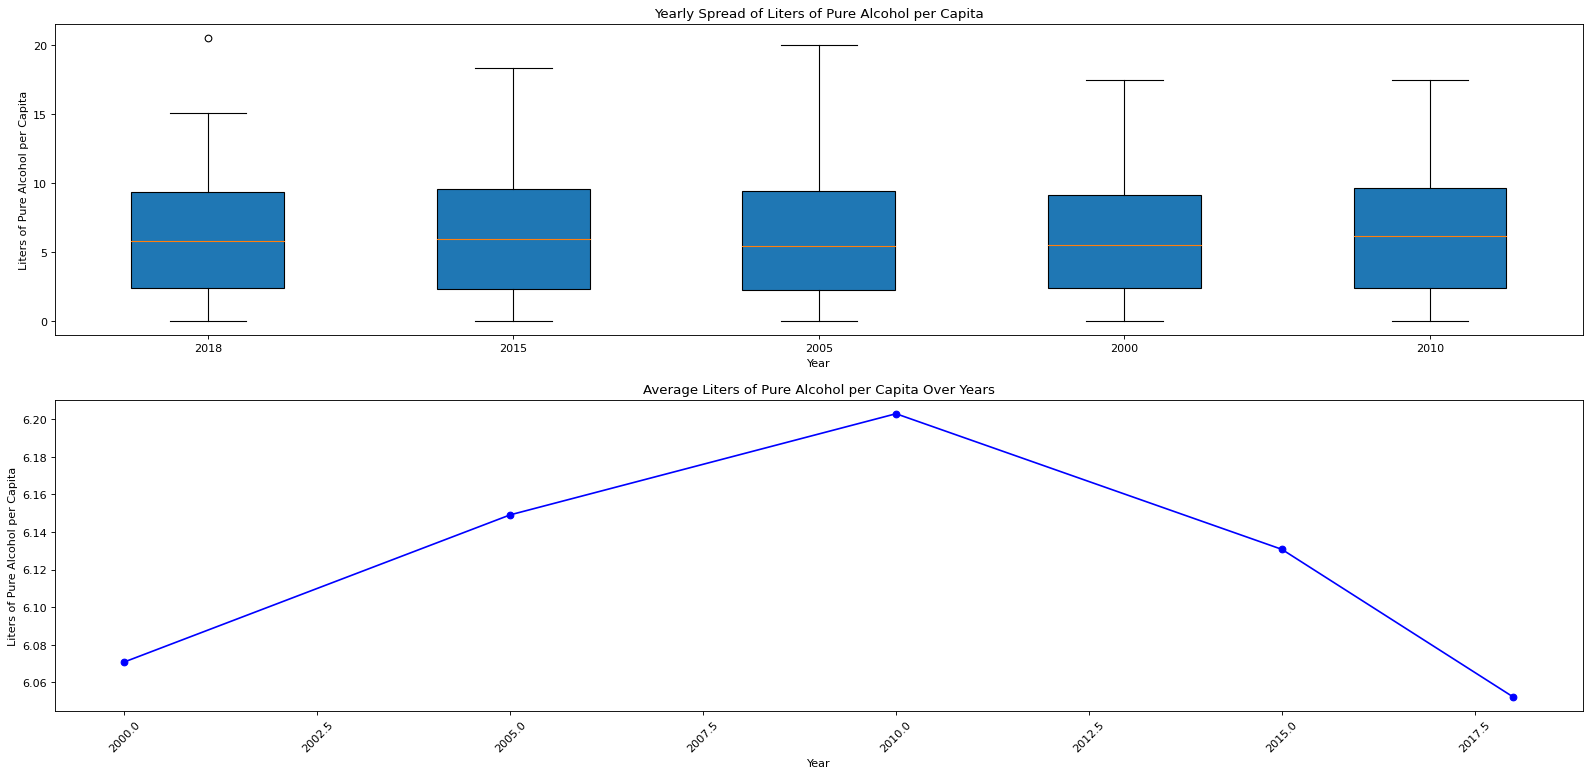
\includegraphics[scale=0.3]{images/du_alcohol_li_of_pu_al_pe_ca_y_trend}
                \caption{Trend of Liters of pure alcohol consumption per capita over years.}
                \label{fig:du-alcohol-trend-years}
            \end{figure}

            Key insights from the boxplot include:

            \begin{itemize}
                \item \textbf{Peak in 2010:} The mean consumption peaked in the year 2010, with an average of approximately 6.20 liters per capita.

                \item \textbf{General Trend:} Starting from about 6.09 liters in the first year, the mean increased to reach its peak in 2010 and later decreased to below 6.06 liters.

                \item \textbf{Stable Variability:} The size of the boxes, representing the interquartile range (IQR), has remained relatively stable over the years. This indicates that the variability in the data has not seen significant changes.

            \end{itemize}

            The boxplot indicates that there was a temporary increase in alcohol consumption around the year 2010, but this was followed by a decline. The stability of the box sizes suggests that despite fluctuations in the mean, the overall distribution of alcohol consumption has remained relatively constant.

            \figurename~\ref{fig:du-alcohol-distribution} presents a histogram that showcases the distribution of liters of pure alcohol consumed per capita. The data primarily ranges between 0 and about 17 liters, although there are a few instances of consumption reaching approximately 20 liters.

            \begin{figure}[H]
                \centering
                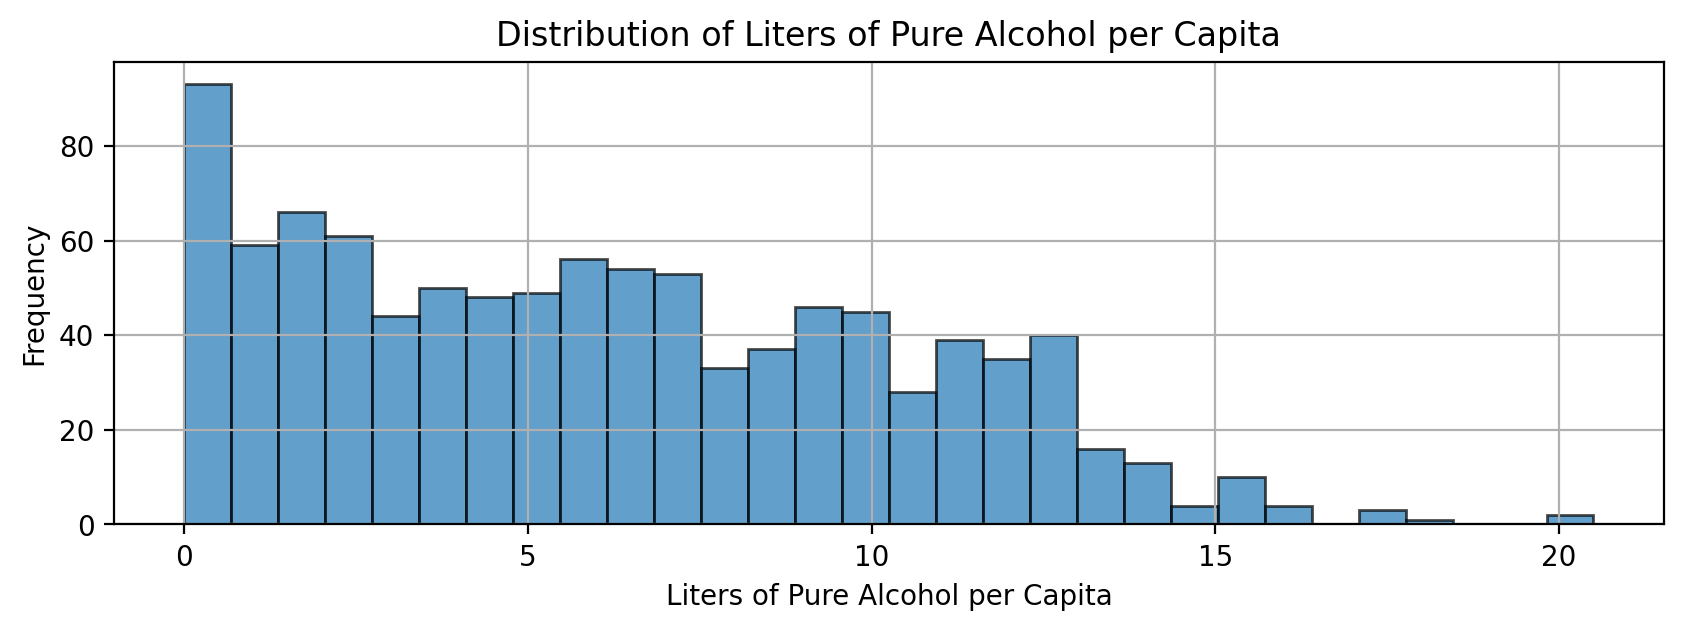
\includegraphics[scale=0.8]{images/du_alcohol_li_of_pu_al_pe_ca_freq}
                \caption{Distribution of consume of pure alcohol in frequency.}
                \label{fig:du-alcohol-distribution}
            \end{figure}

            Key observations from the histogram include:

            \begin{itemize}
                \item \textbf{Peak at Zero:} The histogram peaks just over 0 liters, indicating that a substantial number of data points have near zero alcohol consumption.

                \item \textbf{Main Data Range:} Most of the data is clustered between 0 and approximately 1.5 liters, showing that low levels of alcohol consumption are the most common.

                \item \textbf{Upper Range:} Though the frequencies are low, there are some instances of alcohol consumption reaching around 20 liters.
            \end{itemize}

            The histogram provides an insightful visual representation of alcohol consumption habits. It underscores that while low to moderate alcohol consumption is the norm, there are outliers with substantially higher levels of consumption, which could be of interest for targeted public health initiatives.

            \subsubsection{Statistical Summary of the \dsAlcohol}
                \begin{figure}[H]
                        \centering
                        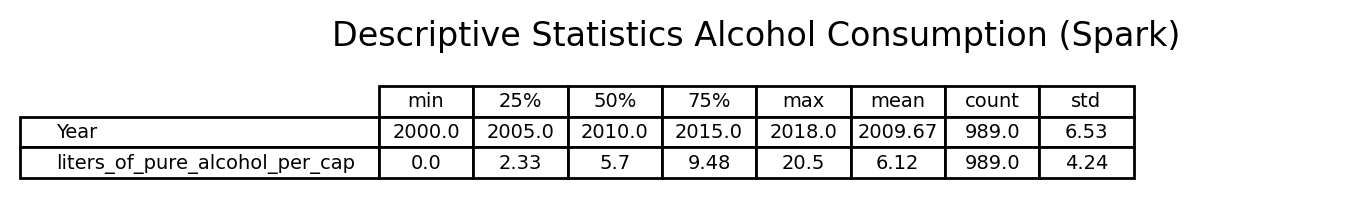
\includegraphics[scale=1]{images/du_alcohol_summary}
                        \caption{}
                        \label{fig:du-alcohol-summary}
                \end{figure}


                The \textit{\dsAlcohol} (\figurename~\ref{fig:du-alcohol-summary}) offers a snapshot of alcohol consumption per capita, captured between the years 2000 and an unspecified recent year. The dataset consists of 989 entries. Below is a straightforward explanation of its key statistics:

                \begin{itemize}
                        \item \textbf{Year:} The dataset covers the years 2000 to 2018, with an average year of about 2010. The standard deviation of 6.53 suggests that the data is relatively evenly distributed over these years.

                        \item \textbf{liters\_of\_pure\_alcohol\_per\_capita:} This metric ranges from 0 to 20.5 liters per capita per year. The average consumption is approximately 6.12 liters, with a standard deviation of 4.24, indicating a notable variation in alcohol consumption rates across the dataset.
                \end{itemize}

                In summary, the dataset provides a comprehensive look into alcohol consumption rates across different time periods, with no missing values in the columns discussed.


    \section{\dsHunger}

        \subsection{\duCollectInitialData}

            Utilizing data from Our World In Data provides convenience, as it provides the flexibility of complete or targeted data downloads. The available presentation formats encompass charts, maps, and tables, which streamline the analysis procedure.
            \\
            \\
            The Global Hunger Index (GHI) functions as an all-encompassing tool to evaluate hunger globally. It combines four indicators to produce a single score, where a higher score indicates deteriorating hunger levels, and a lower score signifies improvement. These indicators encompass undernourishment, child wasting (acute undernutrition), child stunting (chronic undernutrition), and child mortality.
            \\
            \\
            This dataset will serve the purpose of discerning instances where a low percentage is connected to countries with populations that do not experience hunger. This approach is aimed at preventing misinterpretation of results, as countries with low percentages stemming from hunger-related challenges might lead to misguided conclusions regarding crucial variables. Such misinterpretations could potentially distort the genuine patterns and yield inaccurate insights.

        \subsection{\duDescribeTheData}
            \begin{figure}[H]
                \centering
                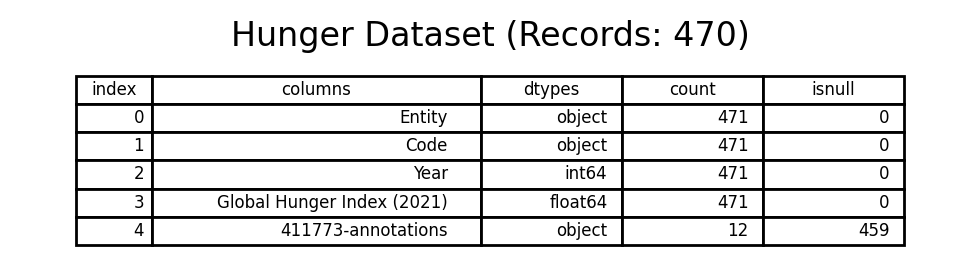
\includegraphics[scale=1.3]{images/du_hunger_dataset}
                \caption{Contains the index of hunger by country and year. Not included countries are not in hunger.}
                \label{fig:du-hunger-datasets}
            \end{figure}
            The \textit{\dsHunger} (\figurename~\ref{fig:du-hunger-datasets}) consists of a total of 471 entries, spread across 5 columns.

            \textbf{Text-based Columns:}
            \begin{enumerate}
                \item \textit{Entity}: Describes the geographical or organizational entity and is complete with no missing values.
                \item \textit{Code}: This column serves as a code or identifier for the entity and also has no missing values.
                \item \textit{411773-annotations}: Contains annotations or additional information, but it is mostly missing data, with only 12 entries filled.
            \end{enumerate}

            \textbf{Numerical Columns:}
            \begin{enumerate}
                \item \textit{Year}: An integer column indicating the year of the data, with no missing entries.
                \item \textit{Global Hunger Index (2021)}: A float column that presumably measures the Global Hunger Index for the year 2021, and it has no missing values.
            \end{enumerate}

            In summary, most columns in the dataset are complete except for \textit{411773-annotations}, which has a significant number of missing entries.

        \subsection{\duExploreTheData}
            \begin{figure}[H]
                \centering
                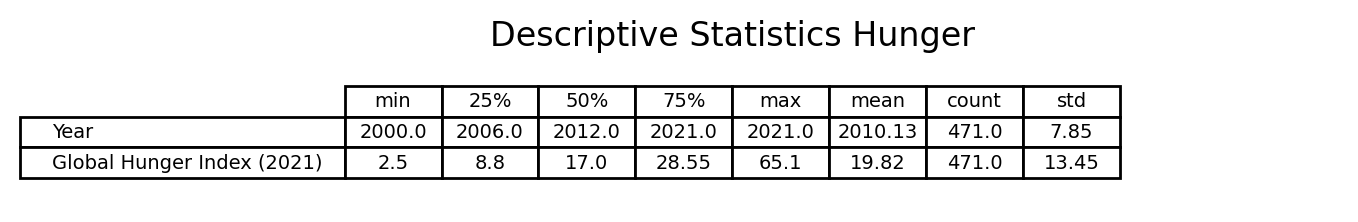
\includegraphics[scale=1]{images/du_hunger_summary}
                \caption{}
                \label{fig:du-hunger-summary}
            \end{figure}

            \subsubsection{Statistical Summary of \dsHunger}

                The \textit{\dsHunger} (\figurename~\ref{fig:du-hunger-summary}) contains data on global hunger, collected between the years 2000 and a more recent year not specified in the summary. With 471 total entries, the dataset gives us several important statistics:

                \begin{itemize}
                        \item \textbf{Year:} The dataset spans from the year 2000 to 2021. The average year of the data is approximately 2010, with a standard deviation of 7.85, indicating that the data is fairly evenly distributed over this time period.

                        \item \textbf{Global Hunger Index (2021):} The Global Hunger Index scores range from a minimum of 2.5 to a maximum of 65.1. The average score stands at 19.82, indicating moderate levels of hunger globally. The standard deviation of 13.45 suggests significant variability in the hunger index scores across different data points.
                \end{itemize}

                In summary, the dataset provides a good understanding of the temporal distribution of global hunger metrics, with no missing values in the columns reviewed.


                \figurename~\ref{fig:du-hunger-countries-top-lw-20} features two vertically arranged boxplots, each providing insight into the Global Hunger Index in different sets of countries. The top boxplot is focused on countries with the highest levels of hunger, whereas the bottom boxplot covers countries with the lowest levels. This data ranges from the year 2000 to 2021.

                \begin{figure}[H]
                        \centering
                        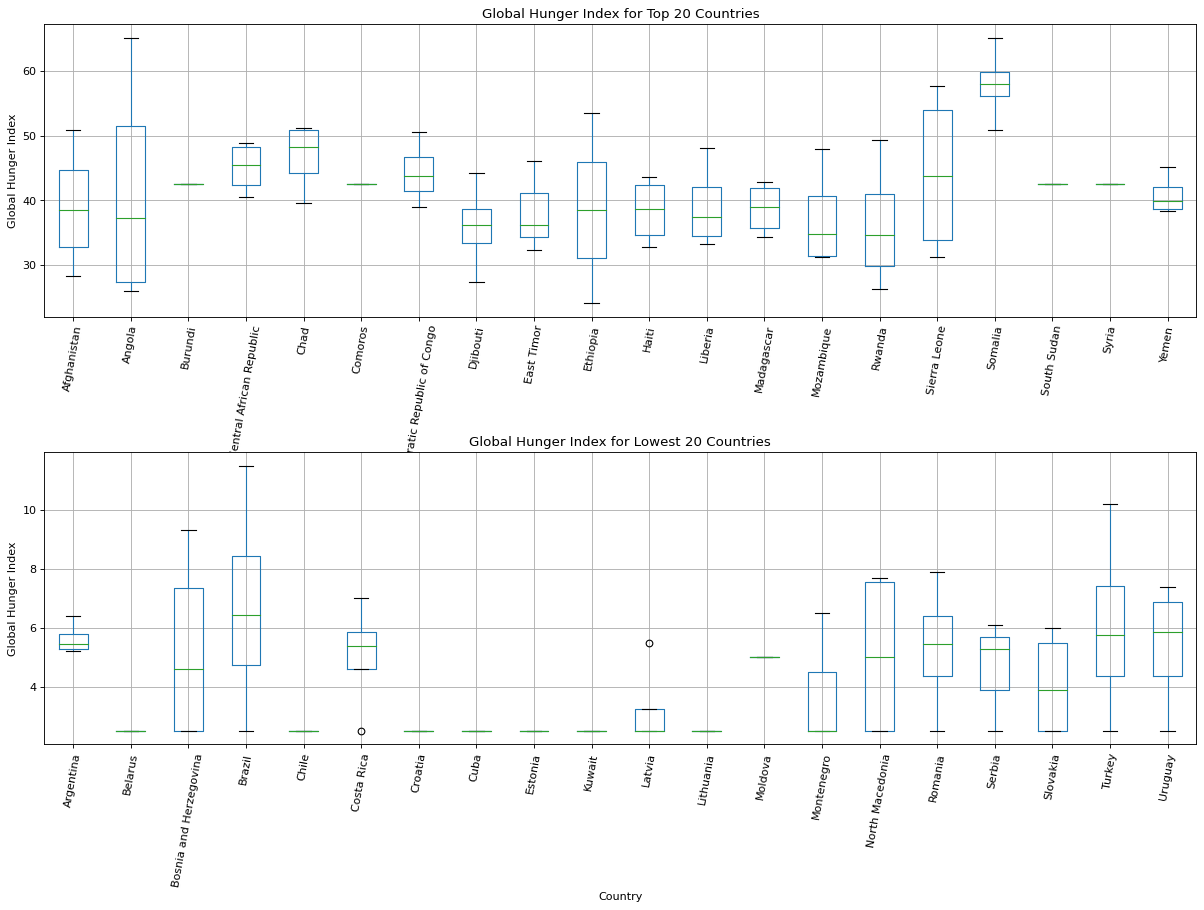
\includegraphics[scale=0.4]{images/du_hunger_hu_in_cou_t_l_20}
                        \caption{Hunger Index, 20 top countries at the top, 20 lowest a the button.}
                        \label{fig:du-hunger-countries-top-lw-20}
                \end{figure}

                The main observations from these boxplots include:

                \begin{itemize}
                        \item \textbf{Countries with High Hunger Index:} Notably, Somalia, Angola, and Sierra Leone are among the countries with the highest levels of hunger according to the Global Hunger Index.

                        \item \textbf{Countries with Low Hunger Index:} On the flip side, countries like Chile, Croatia, and Cuba stand out for their particularly low levels of hunger.

                        \item \textbf{Time Period:} The data envelops a period from 2000 to 2021, allowing for an extensive examination of hunger trends over more than two decades.
                \end{itemize}

                The contrasting boxplots serve as a compelling visualization of the diverse challenges faced by countries when it comes to combating hunger. The data calls attention to the need for targeted interventions that are tailored to the specific circumstances of countries at both ends of the Global Hunger Index.


%                \begin{figure}[H]
%                        \centering
%                        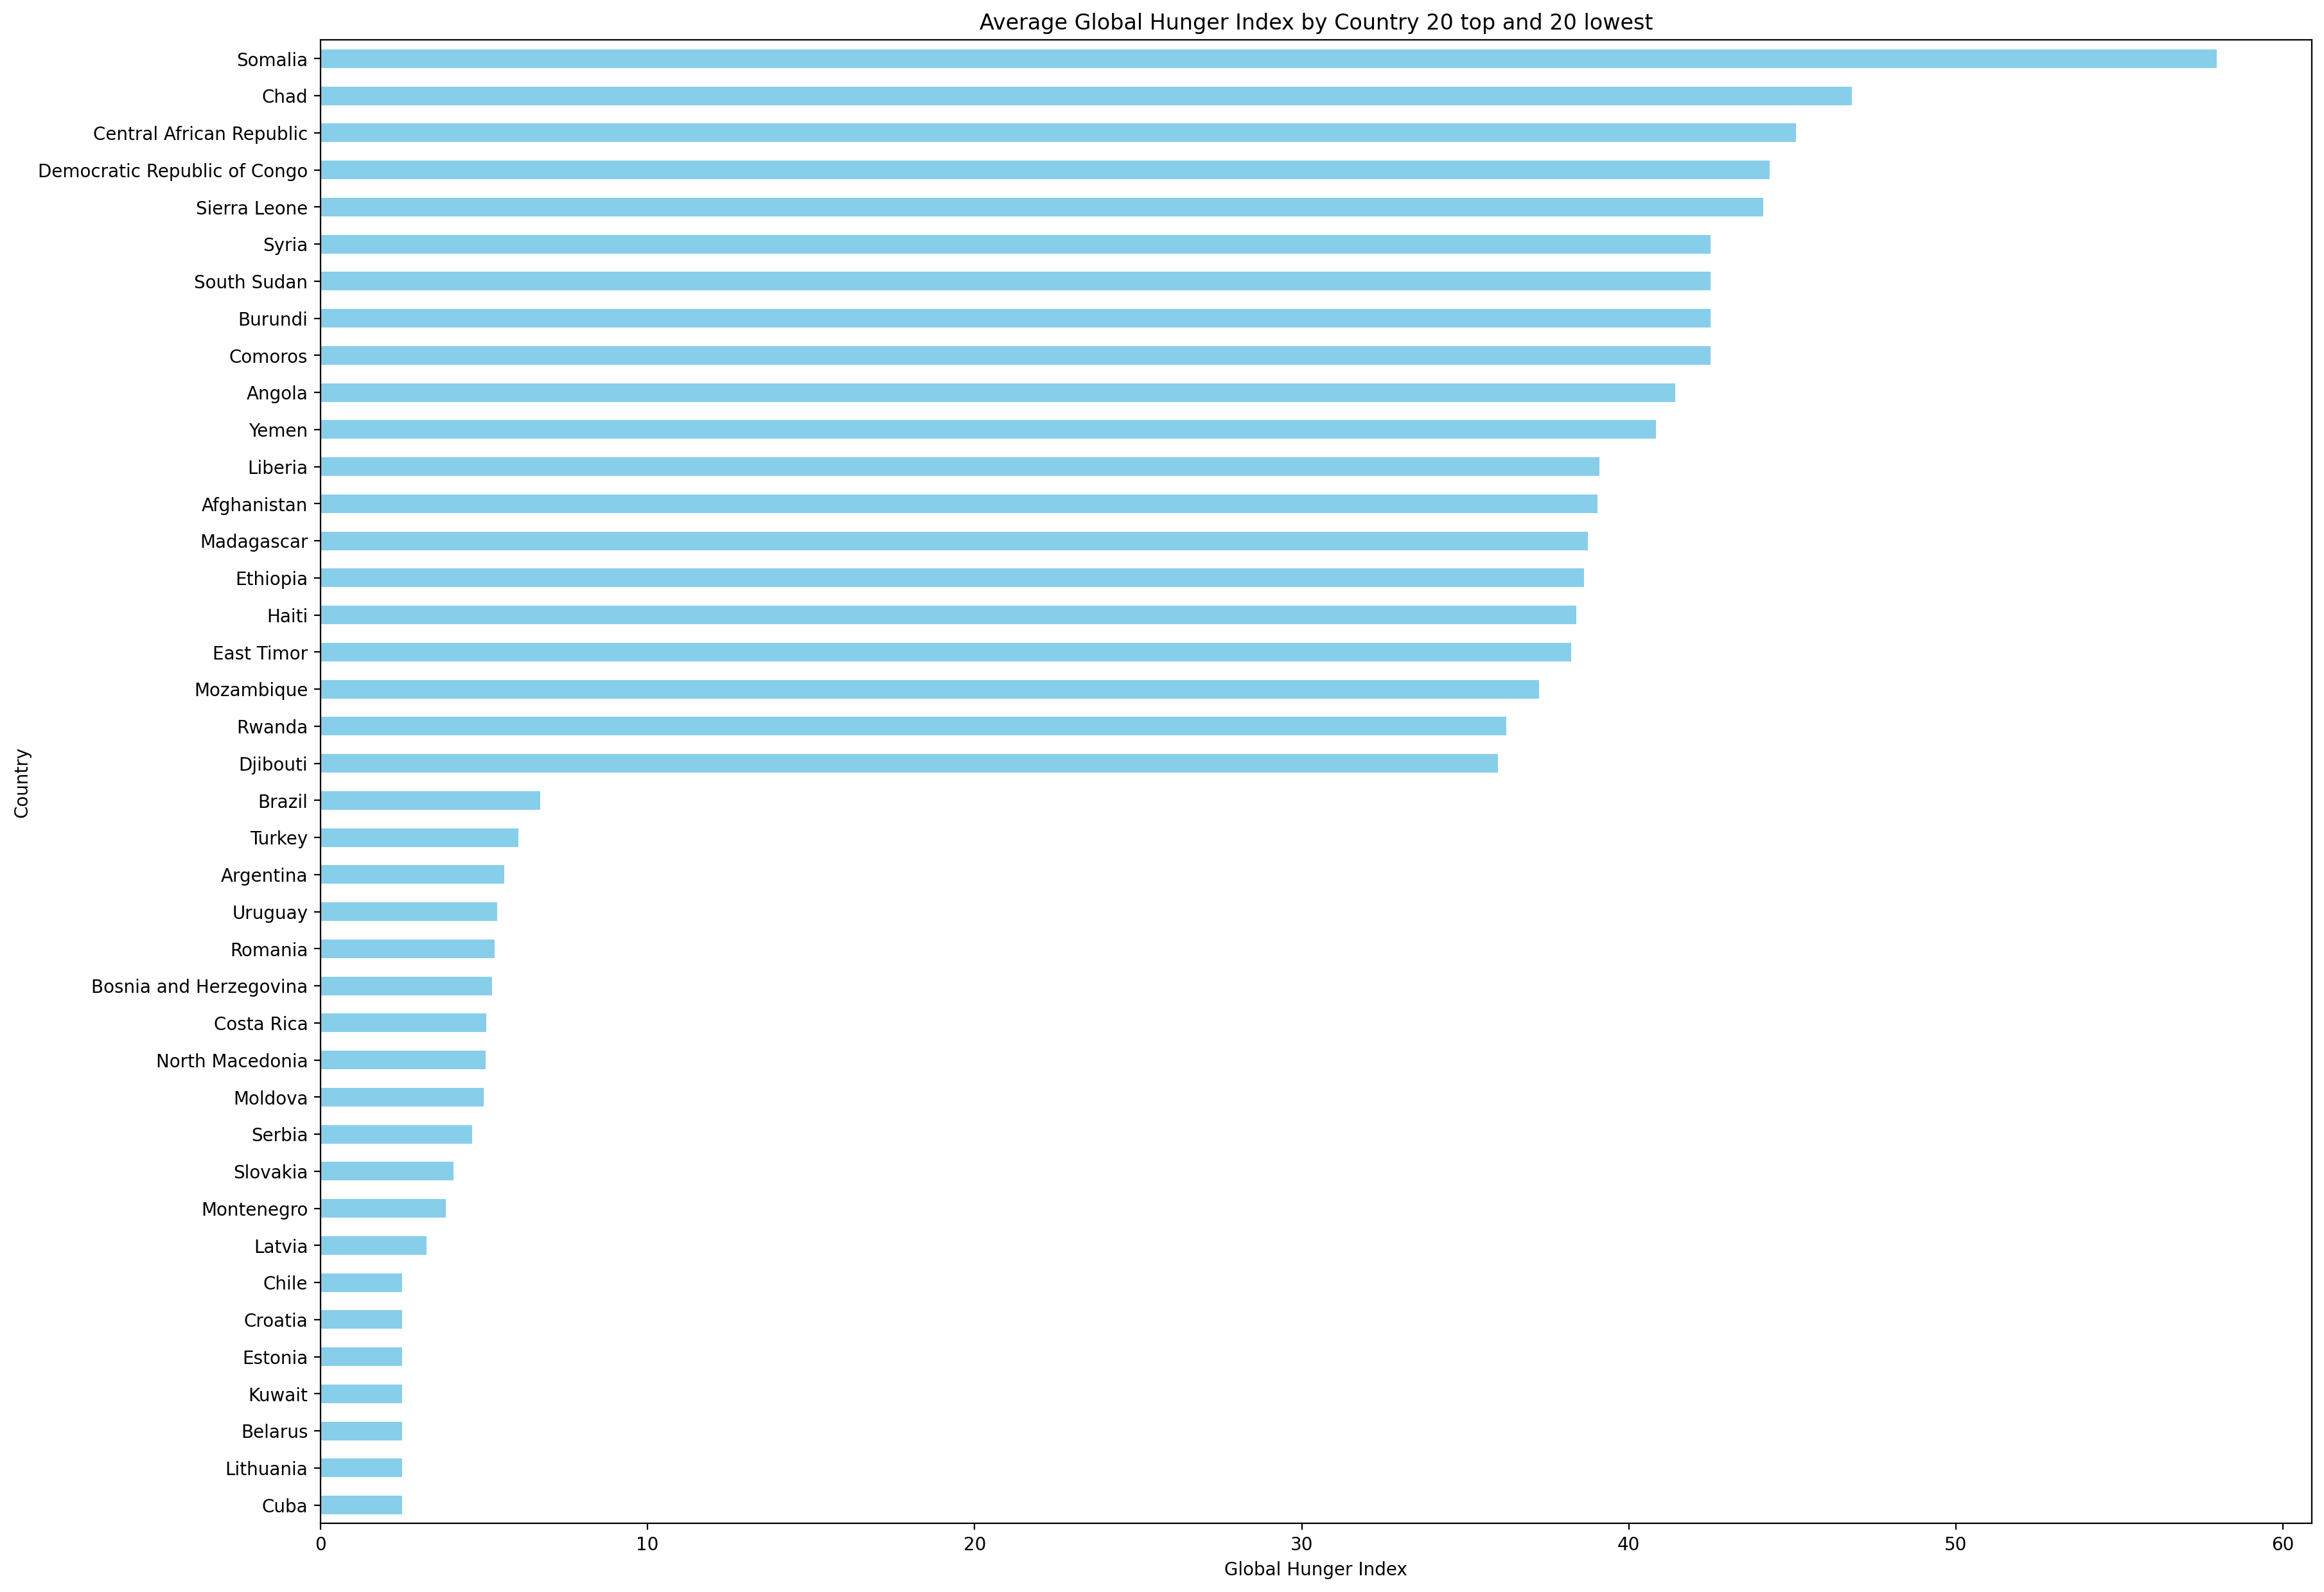
\includegraphics[scale=0.3]{images/du_hunger_hu_in_cou_t_l_20_v2}
%                        \caption{Hunger Index, 20 top and 20 lowest percentages by countries.}
%                        \label{fig:du-hunger-countries-top-ww-20-2}
%                \end{figure}

                \figurename~\ref{fig:du-hunger-trend-years} depicts plots that outlines the distribution of the Global Hunger Index for selected years: 2000, 2005, 2010, 2015, and 2021.


                \begin{figure}[H]
                        \centering
                        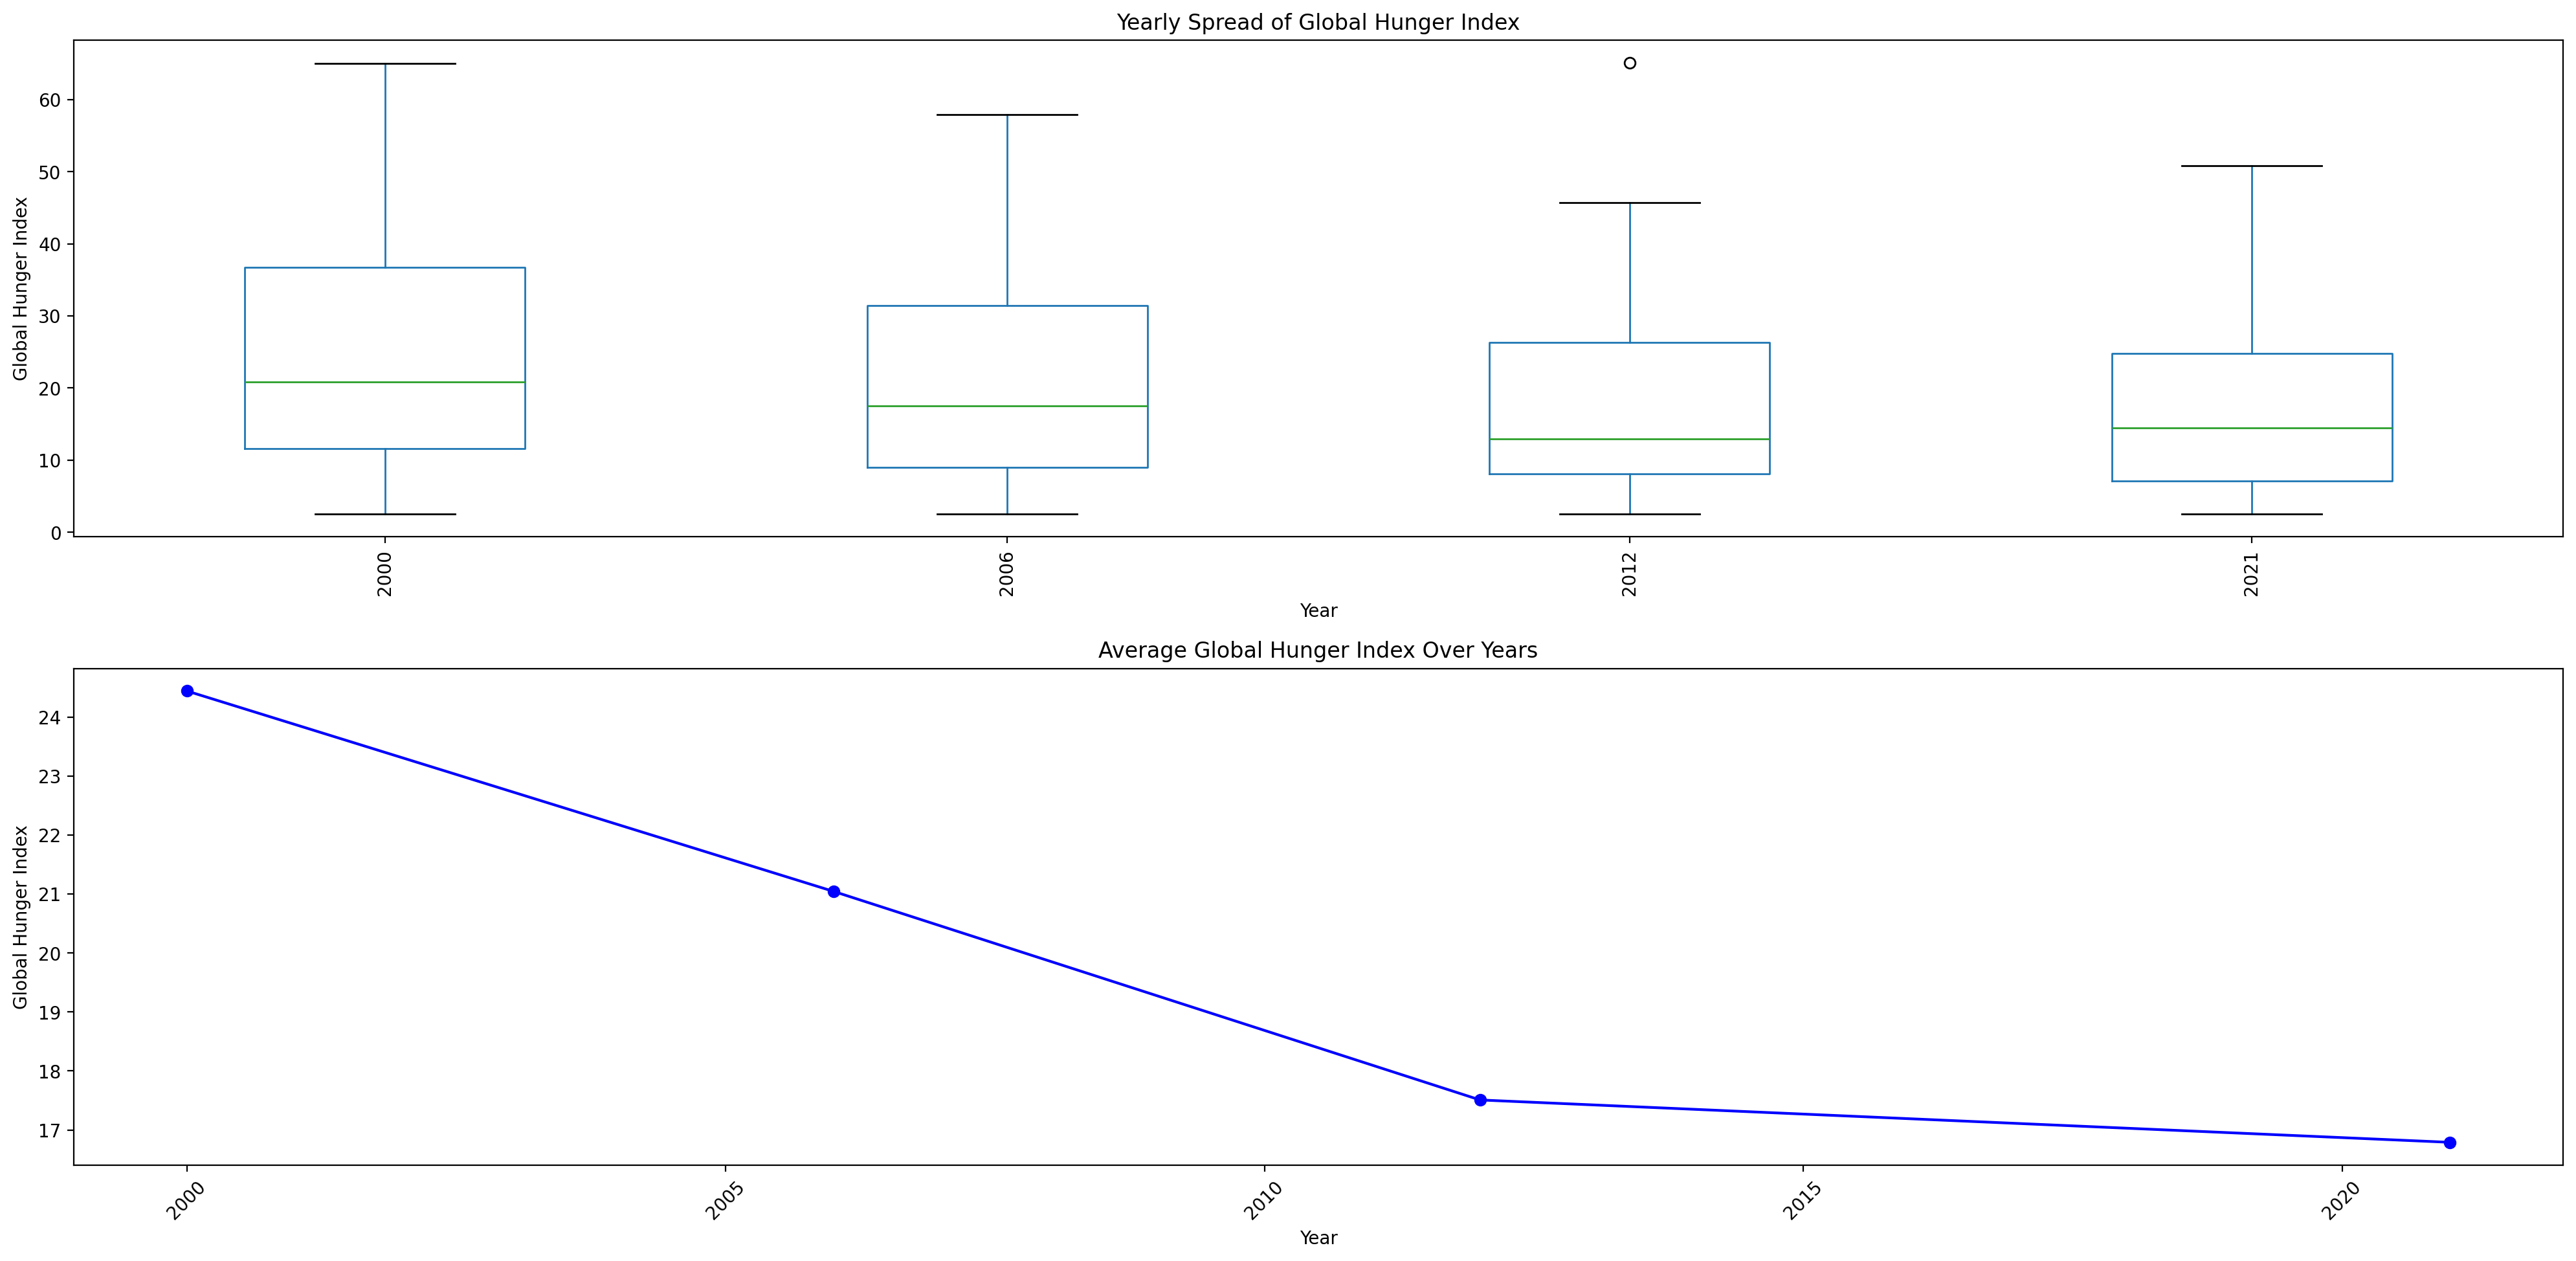
\includegraphics[scale=0.3]{images/du_hunger_hu_in_y_trend}
                        \caption{Trend of Hunger Index over years.}
                        \label{fig:du-hunger-trend-years}
                \end{figure}


                Key observations from the boxplot include:

                \begin{itemize}
                        \item \textbf{Initial High Levels:} The index started at high levels, being over 25 in the year 2000.

                        \item \textbf{Drastic Decrease:} There was a significant drop in the index values by the year 2010, indicating a marked improvement in hunger conditions.

                        \item \textbf{Continued Improvement:} The decreasing trend continued past 2010, extending into 2020, although at a slower pace.

                        \item \textbf{Changes in Maximum Points:} The maximum point in the boxplot was over 60 in 2000, which then decreased to around 50 by 2012. Interestingly, it rose again to above 50 in 2021.
                \end{itemize}

                The boxplot suggests that while there have been significant strides in reducing global hunger, the issue persists with variable severity in different regions, as evidenced by the fluctuating maximum values.


                \figurename~\ref{fig:du-hunger-distribution} presents a histogram depicting the distribution of the Global Hunger Index scores across various countries. The data primarily clusters between 3 and 50, although there are a few rare instances where the index exceeds 60.

                \begin{figure}[H]
                        \centering
                        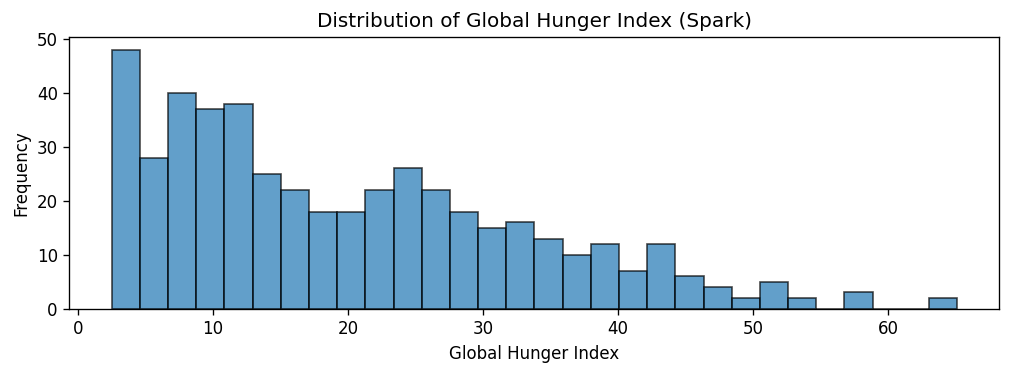
\includegraphics[scale=0.8]{images/du_hunger_hu_in_freq}
                        \caption{Distribution of Hunger Indexes.}
                        \label{fig:du-hunger-distribution}
                \end{figure}


                Key observations from this histogram include:

                \begin{itemize}
                        \item \textbf{Peak at 3:} The histogram peaks around an index score of 3, indicating a substantial portion of the data points fall into this lower hunger range.

                        \item \textbf{Primary Data Cluster:} The bulk of the data falls between 3 and approximately 50, suggesting that moderate levels of hunger are most common among the countries represented.

                        \item \textbf{Outlying High Scores:} Though they are rare, there are a few instances where the Global Hunger Index scores rise above 60.
                \end{itemize}

                The histogram serves as a compelling representation of the various levels of hunger experienced around the world. It emphasizes that although moderate levels of hunger are most common, there are outliers with extremely high levels of hunger that warrant special attention for humanitarian intervention.


    \section{\dsSmoking}

        \subsection{\duCollectInitialData}

            Drawing upon data from Our World In Data provides a valuable convenience, granting users the flexibility to opt for either broad or targeted data downloads. The array of presentation formats, spanning charts, maps, and tables, significantly streamlines the analysis process.
            \\
            \\
            Within this dataset, the consumption of diverse tobacco products is covered, encompassing items such as cigarettes, waterpipes, bidis, pipes, cigars, kretek, heated tobacco products. Oral/nasal smokeless variants as well. Notably, exclusions consist of e-cigarettes, e-hookahs, e-pipes, and e-cigars.

        \subsection{\duDescribeTheData}
            \begin{figure}[H]
                \centering
                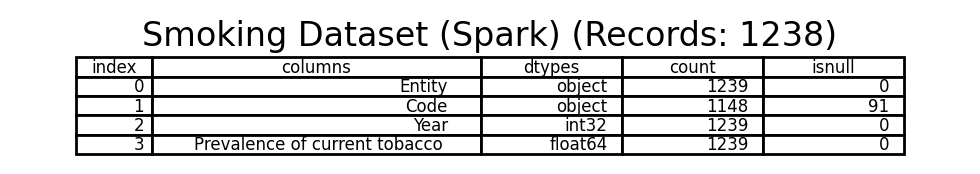
\includegraphics[scale=1.3]{images/du_smoking_dataset}
                \caption{Contains the percentage of prevalence of smoking by country and year}
                \label{fig:du-smoking-datasets}
            \end{figure}

            The \textit{\dsSmoking} (\figurename~\ref{fig:du-smoking-datasets}) contains a total of 1,239 entries and is organized into 4 columns.

            \textbf{Text-based Columns:}
            \begin{enumerate}
                \item \textit{Entity}: This column describes the geographical or organizational entity and has no missing values.
                \item \textit{Code}: Serves as a code or identifier for the entity but has 91 missing entries.
            \end{enumerate}

            \textbf{Numerical Columns:}
            \begin{enumerate}
                \item \textit{Year}: An integer column that specifies the year of data collection. It is complete with no missing values.
                \item \textit{Prevalence of current tobacco use (\% of adults)}: This is a float column that measures the percentage of adults who currently use tobacco. It has no missing entries.
            \end{enumerate}

            In summary, the dataset is almost entirely complete. The only column with missing data is \textit{Code}, which lacks 91 entries.

        \subsection{\duExploreTheData}
            \begin{figure}[H]
                \centering
                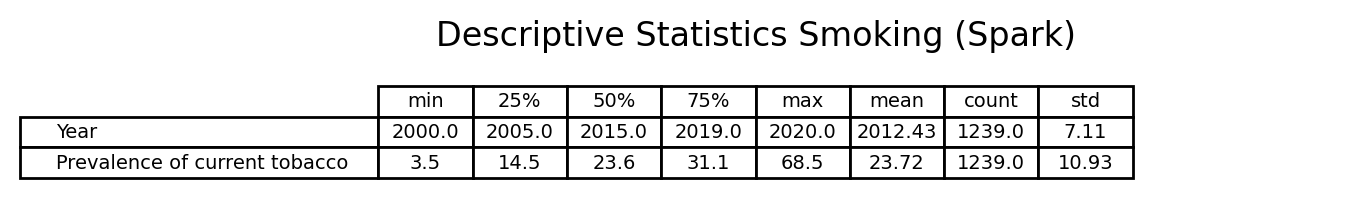
\includegraphics[scale=1]{images/du_smoking_summary}
                \caption{}
                \label{fig:du-smoking-summary}
            \end{figure}


            \figurename~\ref{fig:du-smoking-countries-top-lw-20} contains two vertically aligned boxplots. The top boxplot represents the prevalence of tobacco use among adults in countries with the highest rates, while the bottom boxplot depicts the same for countries with the lowest rates. The data is collected over a span from 2000 to 2020.

            \begin{figure}[H]
                \centering
                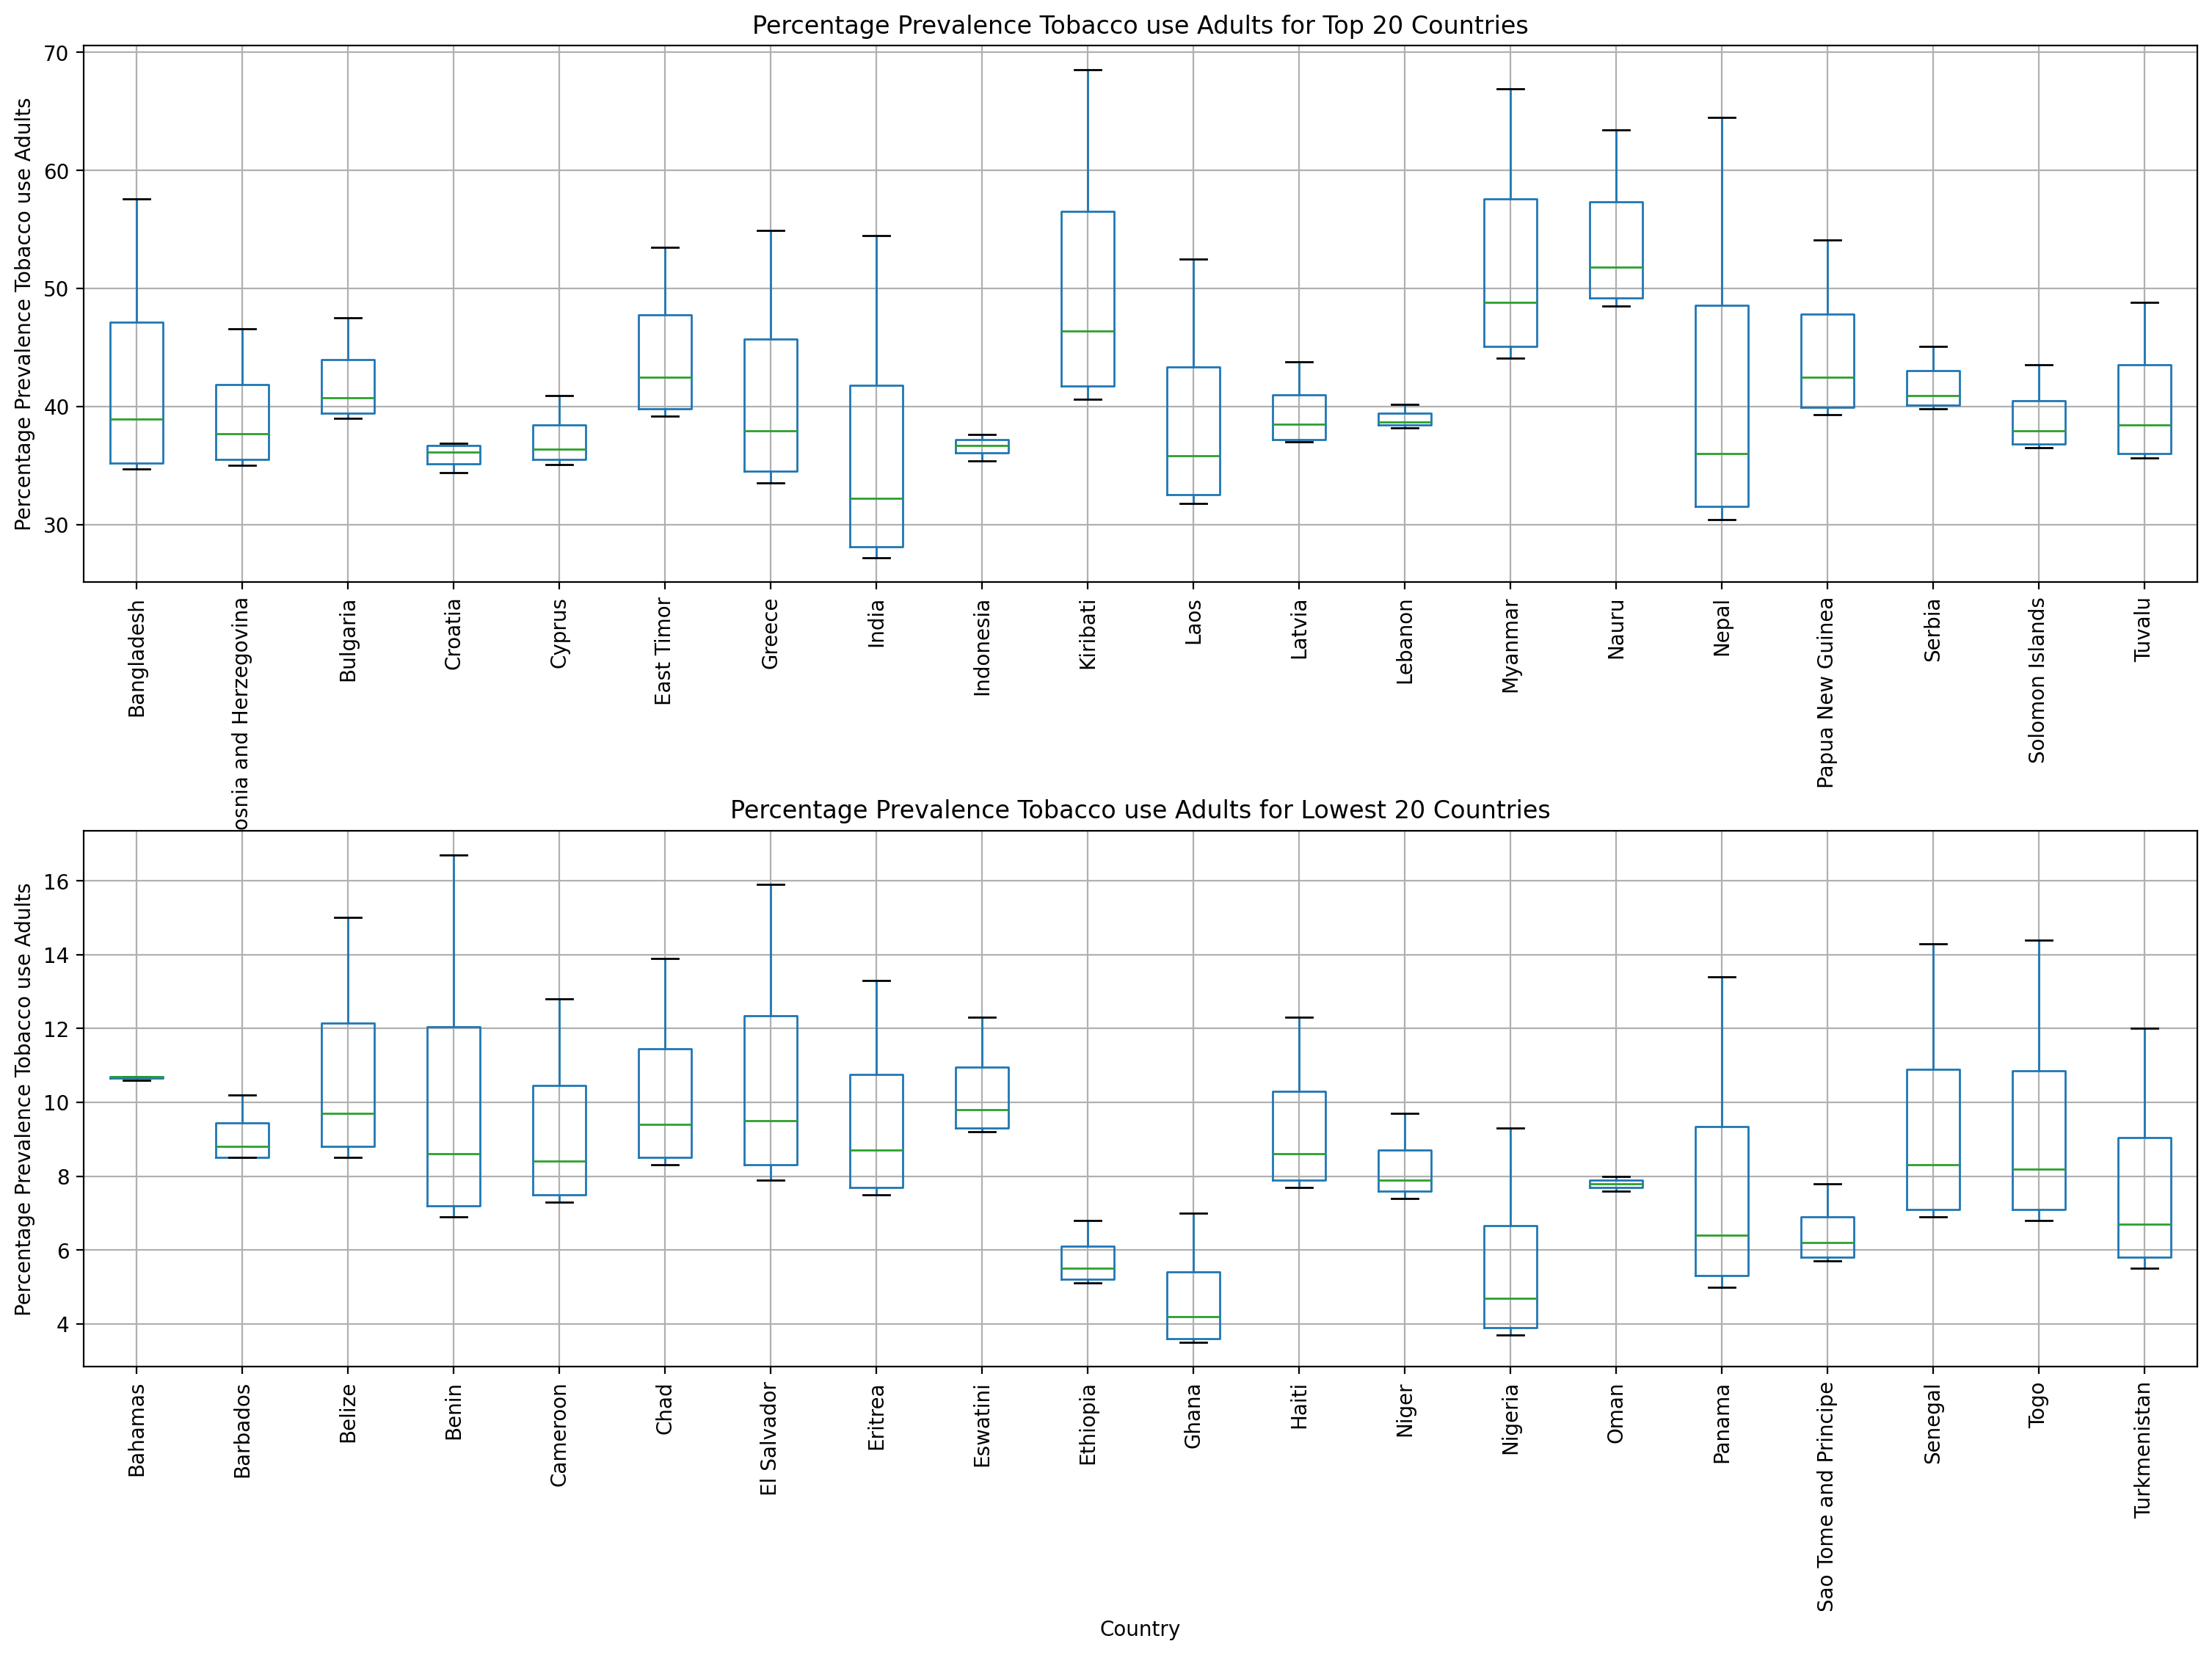
\includegraphics[scale=0.4]{images/du_smoking_pr_sm_cou_t_l_20}
                \caption{\% Prevalence of smoking, 20 top countries at the top, 20 lowest a the button.}
                \label{fig:du-smoking-countries-top-lw-20}
            \end{figure}

            Key takeaways from these boxplots include:

            \begin{itemize}
                \item \textbf{High Prevalence Countries:} Myanmar, Kiribati, and Nauru are noticeably among the countries with the highest prevalence of adult tobacco use.

                \item \textbf{Low Prevalence Countries:} Conversely, countries like Ghana, Nigeria, and Sao Tome and Principe have remarkably low rates of adult tobacco use.

                \item \textbf{Time Frame:} The data encompasses the years from 2000 to 2020, providing an in-depth look at trends in adult tobacco use over a period of two decades.
            \end{itemize}

            The juxtaposition of these boxplots serves to emphasize the substantial differences in adult tobacco use across various countries. The data illuminates the need for specialized public health initiatives that consider the unique challenges each country faces in terms of tobacco consumption.


%            \begin{figure}[H]
%                \centering
%                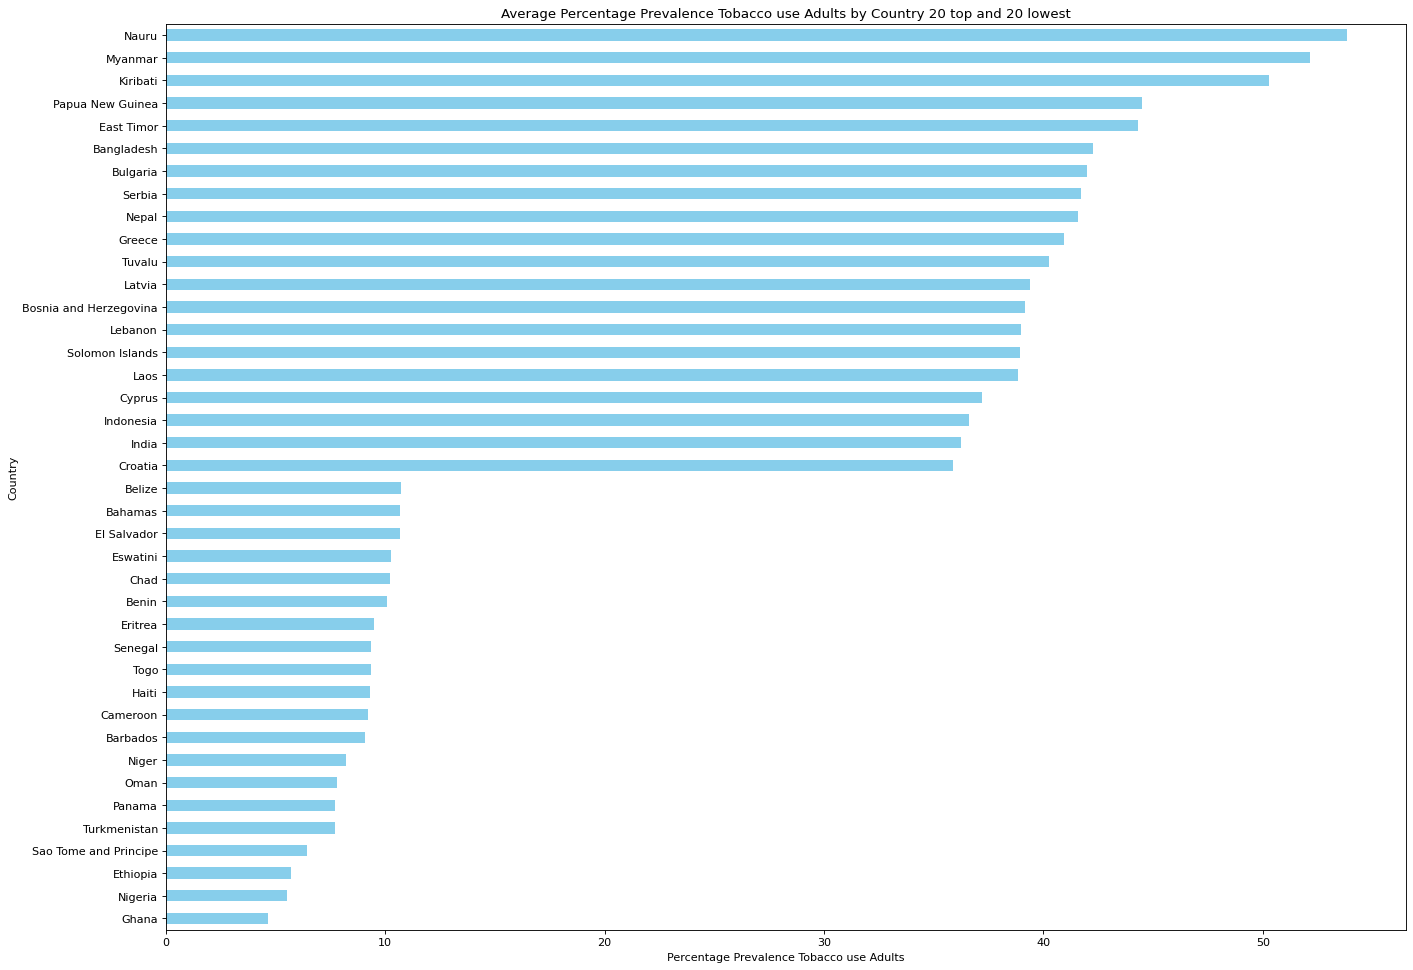
\includegraphics[scale=0.3]{images/du_smoking_pr_sm_cou_t_l_20_v2}
%                \caption{\% Prevalence of smoking, 20 top and 20 lowest percentages by countries.}
%                \label{fig:du-smoking-countries-top-ww-20-2}
%            \end{figure}

            \figurename~\ref{fig:du-smoking-trend-years} provides a combined visual representation of the prevalence of tobacco use among adults over a span of 20 years, from 2000 to 2020. The figure comprises a boxplot as well as a line plot for a more nuanced understanding.

            \begin{figure}[H]
                \centering
                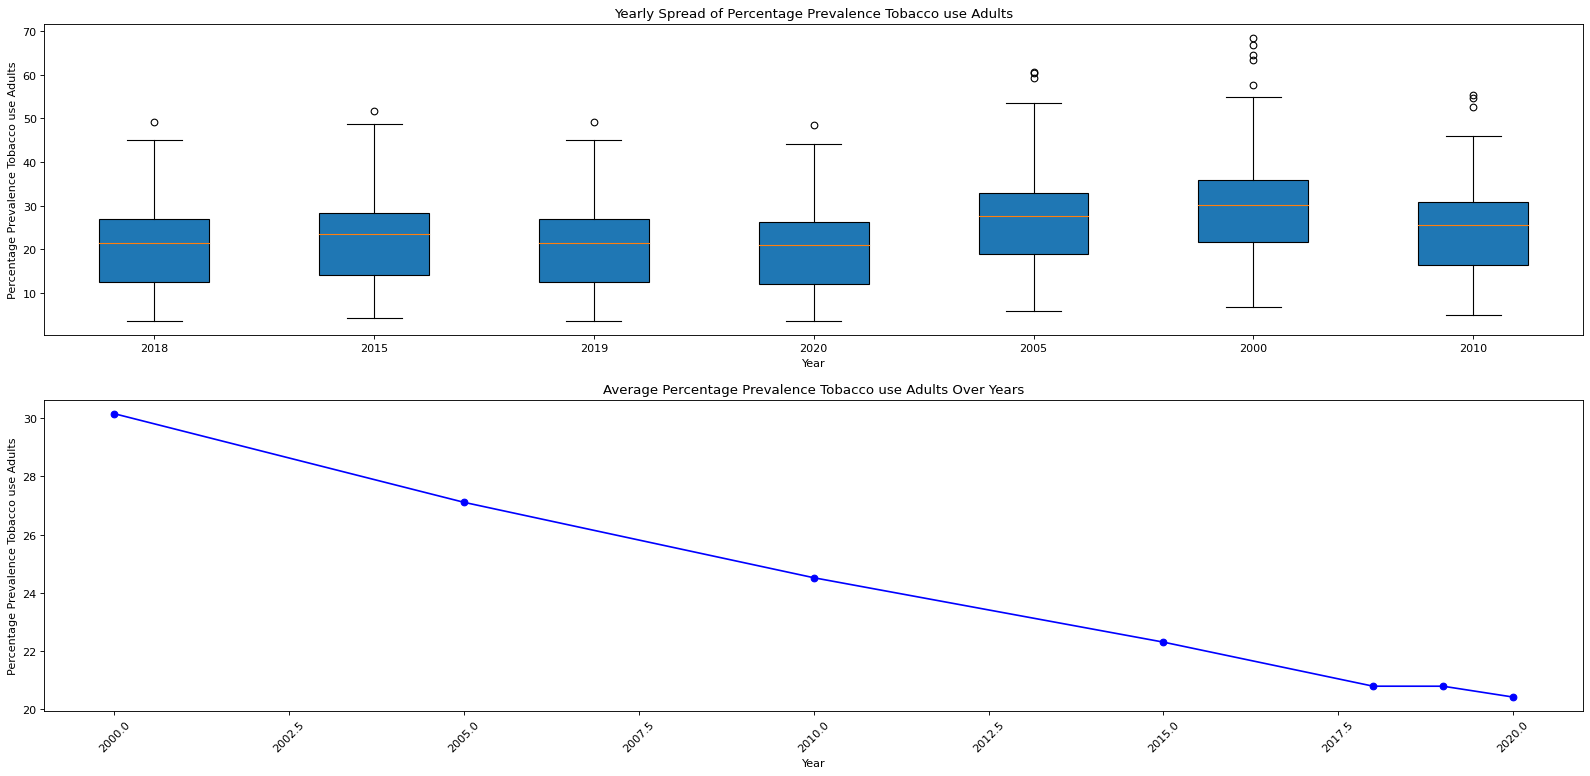
\includegraphics[scale=0.3]{images/du_smoking_pr_sm_y_trend}
                \caption{Trend of prevalence of smoking over years.}
                \label{fig:du-smoking-trend-years}
            \end{figure}

            Key points highlighted by the boxplot and line plot include:

            \begin{itemize}
                \item \textbf{Dramatic Decrease:} The line plot clearly shows that the prevalence of tobacco use among adults has fallen dramatically over the years, from around 30\% in 2000 to just above 20\% in 2020.

                \item \textbf{Year 2000 Outliers:} The boxplot for the year 2000 displays several outliers, indicating that the data was more dispersed during that time.

                \item \textbf{Declining Means:} The means, represented by the center line inside each box, have consistently decreased over the years, which echoes the findings from the line plot.

                \item \textbf{Well-Distributed Data:} The sizes of the boxes remain relatively uniform over the years, suggesting that the data is well-distributed around the mean, despite the overall decline in tobacco use.
            \end{itemize}

            This combined figure provides a comprehensive view of the decreasing trend in tobacco use among adults over the past two decades. The presence of outliers in earlier years and the consistent reduction in mean values emphasize the effectiveness of tobacco control measures over time.


            \figurename~\ref{fig:du-smoking-distribution} shows a histogram outlining the distribution of the prevalence of tobacco use among adults. The data primarily clusters between 4\% and 40\%, with noticeable peaks at around 14\% and 24\%. There are also some rare instances where the prevalence reaches as high as 70\%.

            \begin{figure}[H]
                \centering
                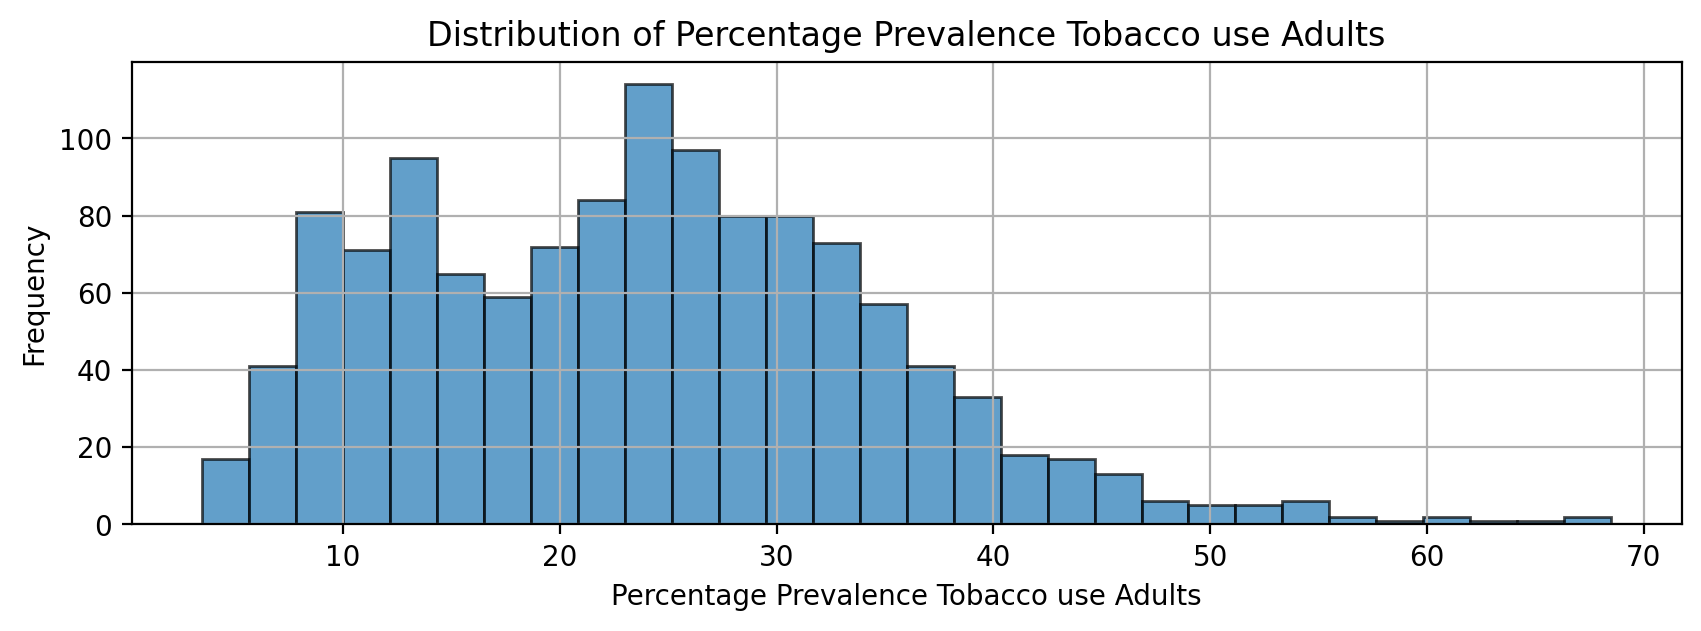
\includegraphics[scale=0.8]{images/du_smoking_pr_sm_freq}
                \caption{Distribution of prevalence of smoking.}
                \label{fig:du-smoking-distribution}
            \end{figure}

            Key insights from the histogram are as follows:

            \begin{itemize}
                \item \textbf{Two Peaks:} The histogram shows two significant peaks, one at around 14\% and another at approximately 24\%, indicating two common levels of adult tobacco use.

                \item \textbf{Main Data Cluster:} The majority of the data is situated between 4\% and 40\%, demonstrating that most countries have moderate levels of adult tobacco use.

                \item \textbf{Rare High Prevalence:} There are a few rare cases where the prevalence of tobacco use spikes to around 70\%.
            \end{itemize}

            The histogram offers a rich visual summary of the varying levels of tobacco use across different countries. It highlights the existence of moderate-to-high levels of tobacco use, and points out that there are a few outlier countries with exceptionally high rates that could be targeted for public health interventions.

            \subsubsection{Statistical Summary of \dsSmoking}

                The \textit{\dsSmoking} (\figurename~\ref{fig:du-smoking-summary}) provides key insights into tobacco usage among adults, capturing data between the years 2000 and an unspecified recent year. The dataset contains 1,239 entries in total. Here's a simple description of its key statistics:

                \begin{itemize}
                        \item \textbf{Year:} The data spans from the year 2000 to 2020. The average year for the dataset is around 2012, and the standard deviation of 7.11 suggests that the data is fairly evenly distributed across this time frame.

                        \item \textbf{Prevalence of current tobacco use (\% of adults):} The dataset records tobacco use prevalence rates ranging from a low of 3.5\% to a high of 68.5\%. The average rate is approximately 23.72\%, with a standard deviation of 10.93, indicating a significant variation in tobacco use across the dataset.
                \end{itemize}

                In summary, the dataset offers a well-rounded view of tobacco use among adults over the years, with no missing values in the columns provided.


    \section{\dsCountries}

        \subsection{\duCollectInitialData}
            The dataset originates from Kaggle and encompasses essential information such as country names, corresponding
            codes, and other pertinent country-related metadata. This dataset assumes the role of a master table, serving
            as a reference for comparisons, merges, and ensuring uniformity of country names across all associated tables.

        \subsection{\duDescribeTheData}
            \begin{figure}[H]
                \centering
                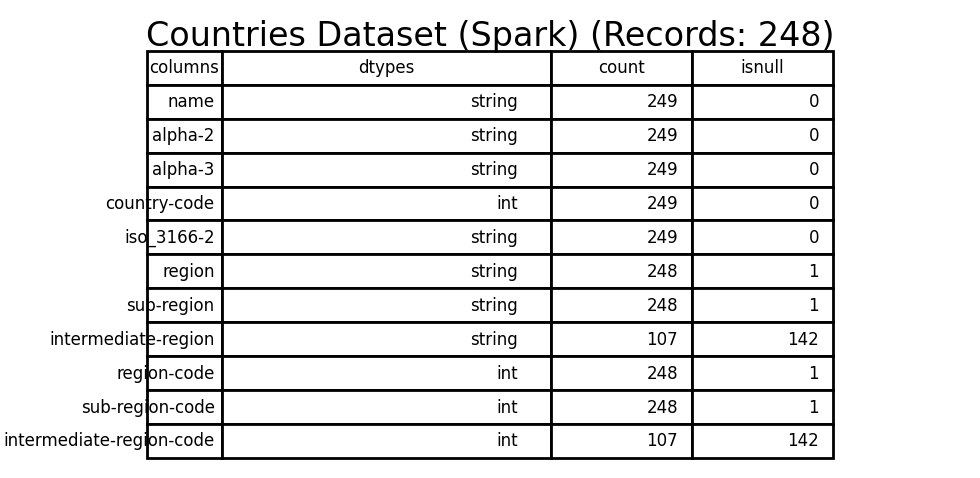
\includegraphics[scale=1.3]{images/du_country_dataset}
                \caption{Contains the codes and country names that will be used to join the tables.}
                \label{fig:du-countries-datasets}
            \end{figure}

            The \textit{\dsCountries} (\figurename~\ref{fig:du-countries-datasets}) is a table containing information on 249 countries. The table is organized into 11 columns.

            \textbf{Text-based Columns:}
            \begin{enumerate}
                \item \textit{name}: Lists the name of the country and has no missing values.
                \item \textit{alpha-2}: Provides a 2-letter country code and has one missing value.
                \item \textit{alpha-3}: Offers a 3-letter country code and has no missing entries.
                \item \textit{iso\_3166-2}: Contains the ISO 3166-2 code and has no missing values.
                \item \textit{region}: Indicates the region to which a country belongs, with one missing value.
                \item \textit{sub-region}: Indicates the sub-region and also has one missing value.
                \item \textit{intermediate-region}: Contains information on the intermediate region, but many entries are missing as only 107 are filled.
            \end{enumerate}

            \textbf{Numerical Columns:}
            \begin{enumerate}
                \item \textit{country-code}: This integer column likely contains unique numerical codes for each country and has no missing values.
                \item \textit{region-code}: This float column likely correlates with the \textit{region} text column and has one missing value.
                \item \textit{sub-region-code}: Similar to \textit{region-code}, this float column likely correlates with \textit{sub-region} and has one missing value.
                \item \textit{intermediate-region-code}: This float column has many missing entries, with only 107 filled.
            \end{enumerate}

            In summary, most columns have complete or nearly complete data, except for \textit{intermediate-region} and \textit{intermediate-region-code}, which have many missing values.

        \subsection{\duExploreTheData}

            The dataset provides an exhaustive list of country names and corresponding codes, which are of utmost
            importance within its scope.
            \\
            \\
            To anticipate potential challenges in integrating multiple sources, a thorough analysis of missing countries
            in each dataset is conducted. \figurename~\ref{fig:du-missing-countries-per-datasets-head-20} displays
            the absent countries (as shown in the left column) for specific datasets. This data will guide the efforts
            in addressing and resolving integration discrepancies related to these countries.
            \begin{figure}[H]
                \centering
                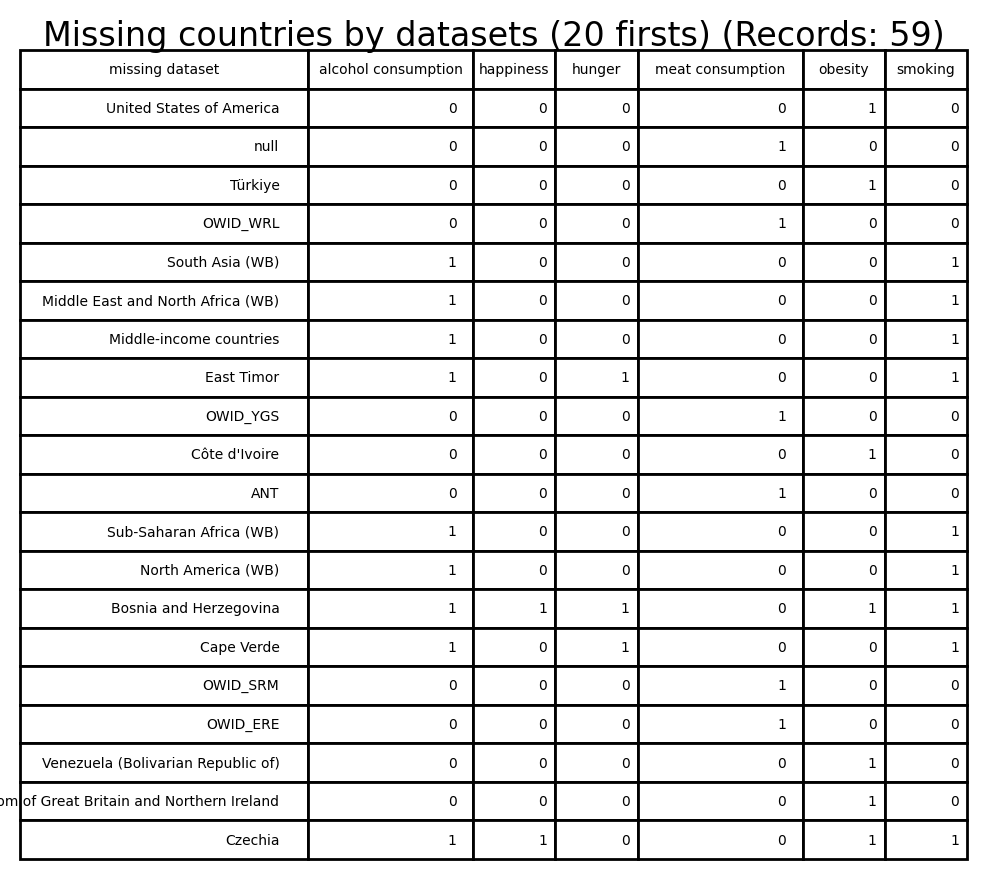
\includegraphics[scale=1.3]{images/du_missing_countries_per_dataset_head_20}
                \caption{Contains the countries that are missing in each dataset, a term per dataset.}
                \label{fig:du-missing-countries-per-datasets-head-20}
            \end{figure}


    \section{Where to find this phase in the code?}

        The is a file, inside the folder python, called iteration\_three.py.
        \\
        \\
        In the line 849 there is a method that execute the whole workflow.

        \begin{verbatim}
            country_manager = ProjectManager(
                generate_images_du_02=True,
            )
            country_manager.du_02()
        \end{verbatim}

        All the images are being generate by code and referenced by using LatEx to create this document.